\documentclass[12pt]{report}
\usepackage[a4paper,margin=1in]{geometry}
\usepackage{setspace} % for single/doublespacing commands
\usepackage{graphicx} % including graphics
\usepackage{sectsty} % sexy section headings
\usepackage{pdfpages} % including multipage pdfs
\usepackage[export]{adjustbox} % for graphic frames and center
\usepackage{amssymb} % special math symbols
\usepackage{cancel} % arrow and cross math cancel symbol
\usepackage[numbered]{matlab-prettifier} % including matlab w/ syntax highlighting
\usepackage[T1]{fontenc} % prettier matlab font
\usepackage[utf8]{inputenc}
\usepackage{circuitikz} % drawing fancy shit
\usepackage{xfrac} % more legible inline fractions (\sfrac)
\usepackage{lmodern} % font package for above
\usepackage{multicol} % multiple columns
\usepackage[justification=centering]{caption} % figure captions (force centering)
\usepackage{amsmath} % more math symbols and shit
\usepackage{enumitem} % add arguments for enumerate to change style
\usepackage{subcaption} % subfigures with list of figure support option [list=true]
\usepackage{BOONDOX-cal} % fancy mathtype script
\usepackage[hidelinks]{hyperref} % clickable table of contents
\hypersetup{
    colorlinks=false, %set true if you want colored links
    linktoc=all,     %set to all if you want both sections and subsections linked
}

\newcommand{\eqname}[1]{\tag*{#1}}% Tag equation with name

\lstMakeShortInline[style=Matlab-editor]| % matlab inline escape character
\usetikzlibrary{arrows,calc,patterns,angles,quotes}
\usetikzlibrary{decorations.pathmorphing,decorations.pathreplacing} % for snakes!
\graphicspath{{images/}}

\allsectionsfont{\centering}
\renewcommand\thesection{\arabic{section}}
\renewcommand{\thefootnote}{\arabic{footnote}}
\setcounter{tocdepth}{2}

\newcommand{\Lag}{\mathcal{L}} % lagrangian L

\begin{document}

\input{titlepage}
\pagenumbering{roman}
{\tableofcontents\let\clearpage\relax\listoffigures}
\clearpage
\pagenumbering{arabic}
\newpage
\begin{flushleft}

% ---------------------------------------------------------------------------- %
\section{Conceptualize the Problem}
% ---------------------------------------------------------------------------- %
\begin{figure}[h]
  \begin{minipage}[c]{.4\textwidth}
  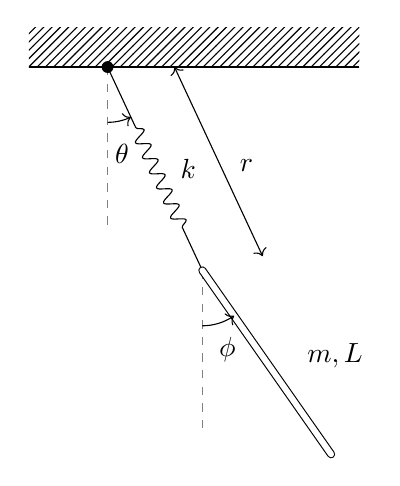
\begin{tikzpicture}

  \pgfmathsetmacro{\Gvec}{1.5}
  \pgfmathsetmacro{\myAngle}{25}

  \coordinate (centro) at (0,0);
  \draw[dashed,gray,-] (centro) -- ++ (0,-2) node (vert1) [black,below]{$ $};

  \draw (centro) -- ++(270+\myAngle:.85) coordinate (spring1);
  \draw[decorate, decoration={snake, segment length=6, amplitude=2.4}] (spring1) -- ++(270+\myAngle:1.5) coordinate (spring);
  \draw (spring) -- ++(270+\myAngle:.5) coordinate (spring2);
  \pic [draw,angle radius=20,->, "$\theta~$", angle eccentricity=1.6] {angle = vert1--centro--spring};

  \draw[<->] (.85,0) -- ++(270+\myAngle:2.65) coordinate (r);
  \draw ($(.85,0) + (270+\myAngle:2.75/2)$) node[label=0:$r$] {};
  \draw ($(.25,0) + (270+\myAngle:2.75/1.5)$) node[label=$k$] {};


  \fill[pattern = north east lines] ($(-1,0)$) rectangle ($(3.2,0.5) $);
  \draw[thick] ($ (centro) + (-1,0) $) -- ($ (centro) + (3.2,0) $);
\draw[dashed,gray,-] (spring2) -- ++ (0,-2) node (vert2) [black,below] {};
  \draw[double distance = .75mm,line cap=round] (spring2) -- ++(270+\myAngle+10:2.85) coordinate (bar);

  \draw ($ (bar) + (.05,1.25)$) node[label] {$m,L$};


  \pic [draw,angle radius=20,->, "$\phi$", angle eccentricity=1.5] {angle = vert2--spring2--bar};

  \fill[black] (centro) circle (0.075);
\end{tikzpicture}

\end{minipage}%
\begin{minipage}[c]{.6\textwidth}
  The pendulum system consists of a rigid bar pinned to the free end of a linear spring,
  which rotates about its opposite end at a fixed point; there are three degrees of freedom,
  since the spring and bar each have an individual angular deflection with respect to the vertical,
  and the radial distance the bar is from the point of rotation due to the variation in the
  length of the spring.
\end{minipage}
\end{figure}

\subsection{Constants and Assumptions}
\begin{tabular}{ll@{\hskip .75in}l}
 \multicolumn{1}{c}{Constants:} && \multicolumn{1}{c}{Assumptions:} \\
 Bar Mass: &$m_b$ = 1 kg & No Losses\\
 Bar Length: &$\ell_b$ = 1 m & Released from Rest\\
 Gravity: &$g$ = 9.81 $\sfrac{\text{m}}{\text{s$^2$}}$ &Uniform Slender Bar \\
 Linear Spring: &&Planar\\
 \quad Spring Coefficient:& $k = 25~\sfrac{\text{N}}{\text{m}}$ &Rigid-Body Dynamics \\
 \quad Unstretched Length:& $\ell_0$ = 0.5 m \\
\end{tabular}
\vspace{5ex}

We are asked to determine the following: \\
\begin{enumerate}
  \item The Equations of Motion for the system via the Lagrangian method.
  \item Integrate the Equations of Motion using various initial conditions and plot
  the behavior of the system for 10 seconds. \\
  \vspace{2ex}
  $
  \begin{array}{cll}
    \text{(a)} & \theta_o = 0~rad, & \phi_o = 0~rad \\
    \text{(b)} & \theta_o = \sfrac{\pi}{18}~rad, & \phi_o = \sfrac{\pi}{9}~rad \\
    \text{(c)} & \theta_o = \sfrac{\pi}{6}~rad, & \phi_o = \sfrac{\pi}{3}~rad \\
  \end{array}
  $
  \item Plot the total energy versus time for all 3 cases.
  \item Repeat 2. and 3. using a '|RelTol|' of $1e-6$ and '|AbsTol|' of $1e-9$ for the
  |ode45| integration tolerances.
\end{enumerate}
\newpage
% ---------------------------------------------------------------------------- %
\section{Free Body Diagram}
% ---------------------------------------------------------------------------- %
\begin{figure}[!htp]
  \caption{Acceleration and Free Body Diagrams}
   \begin{minipage}[c]{.5\textwidth}
     \begin{subfigure}{\textwidth}
       \center
      
\begin{tikzpicture}

  \pgfmathsetmacro{\Gvec}{1.5}
  \pgfmathsetmacro{\myAngle}{25}

  \coordinate (centro) at (0,0);
  \draw[dashed,gray,-] (centro) -- ++ (0,-2) node (vert1) [black,below]{$ $};

  \draw (centro) -- ++(270+\myAngle:.85) coordinate (spring1);
  % \draw[decorate, gray, decoration={snake, segment length=6, amplitude=2.4}]
    % (spring1) -- ++(270+\myAngle:1.5) coordinate(spring);
  % \draw [gray] (spring) -- ++(270+\myAngle:.5) coordinate (spring2);
  \draw[decorate, decoration={snake, segment length=8, amplitude=2.1}]
    (spring1) -- ++(270+\myAngle:1.8) coordinate (springs);
  \draw (springs) -- ++(270+\myAngle:.5) coordinate (springs2);

  \pic [draw,angle radius=20,->, "$\theta~$", angle eccentricity=1.6] {angle = vert1--centro--spring};

  \draw [decorate,decoration={brace,amplitude=2pt,raise=4pt}] (0,0) --
    node [xshift=4.2ex,yshift=1.1ex] {$\ell_0 + \delta$} (springs2);

  % \draw[->] (.85,0) -- ++(270+\myAngle:2.65) coordinate (r);
  % \draw ($(.85,0) + (270+\myAngle:2.75/2)$) node[label=0:$r$] {};
  % \draw ($(.25,0) + (270+\myAngle:2.75/1.5)$) node[label=$k$] {};
  \path (centro) -- node[label={[label distance = 2ex]below:$k$}] (k) {} (spring2);

  \draw [gray,dashed] (-1,0) -- node[above,near end] (datum) {\textit{datum}} (2.5,0);
  \draw[dashed,gray,-] (springs2) -- ++ (0,-2) node (vert2) [black,below] {};
  \draw[double distance = .75mm,line cap=round] (springs2) -- ++(270+\myAngle+10:2.85) coordinate (bar);

  \pic [draw,angle radius=20,->, "$\phi$", angle eccentricity=1.5] {angle = vert2--spring2--bar};

  \coordinate (g) at ($(springs2) + (305:1.425)$);
  \path let \p1 = (g) in node at (\x1,0) (gdatum) {};
  \draw [dashed,gray,-] (g) -- (gdatum);
  \fill[black] (g) circle (0.03);

  % \begin{scope}[shift={(spring2)}]
  %   \draw[gray,dashed,domain=-30:-80] plot ({1.425*cos(\x)}, {1.425*sin(\x)});
  % \end{scope}

  \draw [decorate,decoration={brace,amplitude=2pt,raise=4pt,mirror}] (g) --
    node [xshift=4ex] {$V_{bar}$} (gdatum);

  \draw (g) node[label={[label distance = -1ex]225:$G$}] {};

  \fill[black] (centro) circle (0.075);
\end{tikzpicture}

      \vspace{1ex}
      \caption{Free Body Diagram}
      \label{fbd}
      \end{subfigure}
   \end{minipage}%
   \begin{minipage}[c]{.5\textwidth}
     \begin{subfigure}{\textwidth}
       \center
       \vspace{2ex}
       \begin{tikzpicture}

  \pgfmathsetmacro{\Gvec}{1.5}
  \pgfmathsetmacro{\myAngle}{25}

  \coordinate (centro) at (0,0);
  % \draw[dashed,gray,-] (centro) -- ++ (0,-2) node (vert1) [black,below]{$ $};

  \draw (centro) -- ++(270+\myAngle:.85) coordinate (spring1);
  % \draw[decorate, gray, decoration={snake, segment length=6, amplitude=2.4}]
    % (spring1) -- ++(270+\myAngle:1.5) coordinate(spring);
  % \draw [gray] (spring) -- ++(270+\myAngle:.5) coordinate (spring2);
  \draw[decorate, decoration={snake, segment length=8, amplitude=2.1}]
    (spring1) -- node (middle) {} ++(270+\myAngle:1.8) coordinate (springs);
  \draw (springs) -- ++(270+\myAngle:.5) coordinate (springs2);


  % \draw [decorate,decoration={brace,amplitude=2pt,raise=4pt}] (0,0) --
  %   node [xshift=4.1ex,yshift=1.1ex] {$l_0 + \delta$} (springs2);

  % \draw[->] (.85,0) -- ++(270+\myAngle:2.65) coordinate (r);
  % \draw ($(.85,0) + (270+\myAngle:2.75/2)$) node[label=0:$r$] {};
  % \draw ($(.25,0) + (270+\myAngle:2.75/1.5)$) node[label=$k$] {};
  % \path (centro) -- node[label={[label distance = 2ex]below:$k$}] (k) {} (spring2);

  \draw [gray,dashed] (-1,0) -- node[above,near end] (datum) {\textit{datum}} (2.5,0);
  % \draw[dashed,gray,-] (springs2) -- ++ (0,-2) node (vert2) [black,below] {};
  \draw[double distance = .75mm,line cap=round] (springs2) -- ++(270+\myAngle+10:2.85) coordinate (bar);

  \pic [draw,angle radius=20,->, "$\ddot{\theta}~$", angle eccentricity=1.6] {angle = vert1--centro--spring};

  % \pic [draw,angle radius=20,->, "$\phi$", angle eccentricity=1.5] {angle = vert2--spring2--bar};

  \coordinate (g) at ($(springs2) + (305:1.425)$);
  \pic [draw,->, angle radius=10, angle eccentricity=2,"$\ddot{\phi}$" {yshift=-1ex,xshift=1.5ex}]
  {angle = springs2--g--bar};

  \draw [->] (g) -- node [below,xshift=2ex,yshift=1ex] {$\vec{v}_G$} ++ (35:.75) ;

  \fill[black] (g) circle (0.03);

  \begin{scope}[shift={(springs2)}]
    \draw[gray,dashed,domain=-25:-85] plot ({1.425*cos(\x)}, {1.425*sin(\x)});
  \end{scope}

  \draw [->] ($(.32,0) + (270+\myAngle:3)$) -- node[right,xshift=.5ex,yshift=.5ex]
  {$\ddot{\ell}_s$} ++ (115:.75);
  \draw [-] ($(.1,0) + (270+\myAngle:3.1)$) -- ++ (25:.4);

  % \draw (g) node[label={[label distance = -1ex]225:$G$}] {};

  \fill[black] (centro) circle (0.075);
\end{tikzpicture}

       \vspace{2ex}
       \caption{Acceleration Diagram}
       \label{ad}
    \end{subfigure}
   \end{minipage}
\end{figure}
\vspace{-2ex}
\begin{tabular}{rl@{\hskip .5in}rl}
  $G$:&Center of gravity of the bar &$\vec{v}_G$:& Velocity of bar center of gravity\\
  $\ell_0$:& Spring unstretched length  &$\ddot{\theta}$:& Angular velocity of spring \\
  $\delta$:& Spring deflection &$\ddot{\phi}$:& Angular velocity of bar\\
  $k$:& Spring constant &$\ddot{\ell}_s$:& Radial acceleration of spring \\
  $h_{b}$:& Distance to bar ($G$) from datum \\
  $F_s$:& Force onto bar due to spring\\
  $A_{\theta}$:& Pin reaction in $\theta$ direction\\
  $A_{t}$:& Pin reaction in tangential direction \\
\end{tabular}

% ---------------------------------------------------------------------------- %
\section{Coordinate Frame} \label{section:coord}
% ---------------------------------------------------------------------------- %
\begin{figure}[!htp]
    \begin{minipage}[c]{.4\textwidth}
      \center
      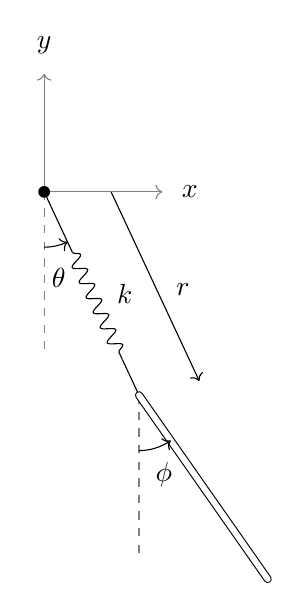
\begin{tikzpicture}

  \pgfmathsetmacro{\Gvec}{1.5}
  \pgfmathsetmacro{\myAngle}{25}

  \coordinate (centro) at (0,0);
  \draw[dashed,gray,-] (centro) -- ++ (0,-2) node (vert1) [black,below]{$ $};

  \draw (centro) -- ++(270+\myAngle:.85) coordinate (spring1);
  \draw[decorate, decoration={snake, segment length=6, amplitude=2.4}] (spring1) -- ++(270+\myAngle:1.5) coordinate (spring);
  \draw (spring) -- ++(270+\myAngle:.5) coordinate (spring2);
  \pic [draw,angle radius=20,->, "$\theta~$", angle eccentricity=1.6] {angle = vert1--centro--spring};

  \draw[->] (.85,0) -- ++(270+\myAngle:2.65) coordinate (r);
  \draw ($(.85,0) + (270+\myAngle:2.75/2)$) node[label=0:$r$] {};
  \draw ($(.25,0) + (270+\myAngle:2.75/1.5)$) node[label=$k$] {};

  \draw[gray,->] (0,0) -- ++ (1.5,0) node (x) {};
  \draw[gray,->] (0,0) -- ++ (0,1.5) node (y) {};
  \draw (x) node[label=east:$x$] {};
  \draw (y) node[label=north:$y$] {};

  \draw[dashed,gray,-] (spring2) -- ++ (0,-2) node (vert2) [black,below] {};
  \draw[double distance = .75mm,line cap=round] (spring2) -- ++(270+\myAngle+10:2.85) coordinate (bar);

  \pic [draw,angle radius=20,->, "$\phi$", angle eccentricity=1.5] {angle = vert2--spring2--bar};

  % \fill[black] ($(spring2) + (305:1.425)$) circle (0.03) coordinate (g);
  % \draw ($(spring2) + (320:1.425)$) node[label] {$G$};

  \fill[black] (centro) circle (0.075);
\end{tikzpicture}

      \caption{Coordinate Frame}
      \label{coord}
      \vspace{2ex}
    \end{minipage}%
    \begin{minipage}[c]{.6\textwidth}
      \center
      \begin{tabular}{rl}
      & \quad Motion Variables: \\
      $\theta$:& Angle of spring relative to vertical\\
      $\phi$:& Angle of bar relative to vertical\\
      $\ell_s$:& Radial length of spring \\
      \\
      & \quad Supplemental Variables: \\
      $\vec{r}_G$:& Vector to bar center of mass from origin \\
    \end{tabular}
    \end{minipage}
\end{figure}
\newpage
% ---------------------------------------------------------------------------- %
\section{Sum of Forces}
% ---------------------------------------------------------------------------- %
From Figure (\ref{coord}),
$$\vec{r}_G = \left[\ell_s\sin(\theta) + \frac{\ell_b}{2}\sin(\phi)\right]\hat{\textrm{\i}}
 + \left[-\ell_s\cos(\theta) - \frac{\ell_b}{2}\cos(\phi)\right]\hat{\textrm{\j}}$$

Taking the time derivative,
$$\frac{d}{dt}\vec{r}_G = \dot{\vec{r}}_G = \vec{v}_G$$
$$
\vec{v}_G =
\left[\dot{\ell}_s\sin(\theta) + \frac{\ell_b\dot{\phi}\cos(\phi)}{2} +
\ell_s\dot{\theta}\cos(\theta)\right]\hat{\textrm{\i}} +
\left[\frac{\ell_b\dot{\phi}\sin(\phi)}{2} -
\dot{\ell}_s\cos(\theta) + \ell_s\dot{\theta}\sin(\theta)\right]\hat{\textrm{\j}}
$$

Kinetic Energy of Spring:
$$T_1 = 0$$
Kinetic Energy of Bar, due to it's rotational and translational velocity (Figure \ref{ad}):
$$T_2 = \frac{1}{2}m_{b}(\vec{v}_G \cdot \vec{v}_G) + \frac{1}{2}I\omega^2$$
Since the moment of inertia $I$ for a uniform slender bar rotating about its end is
$\dfrac{1}{12}m\ell^2$ and $\omega = \dot{\phi}$,
$$T_2 = \frac{1}{2}m_{b}(\vec{v}_G \cdot \vec{v}_G) + \frac{1}{24}m_{b}\ell_b^2\dot{\phi}^2$$
Total Kinetic Energy:
\begin{equation}
T = T_1 + T_2 = \frac{1}{2}m_{b}(\vec{v}_G \cdot \vec{v}_G) + \frac{1}{24}m_{b}\ell_b^2\dot{\phi}^2
\end{equation}

Potential Energy of Spring due to it's stretch (Figure \ref{fbd}):
$$V_1 = \frac{1}{2}k\big(\ell_s-\ell_0\big)^2$$
Potential Energy of Bar, due to it's distance below the datum, $h_{b}$ (Figure \ref{fbd}):
$$V_2 = - m_bg\big(\ell_s\cos(\theta) + \frac{\ell_b}{2}\cos(\phi)\big)$$
Total Potential Energy:
\begin{equation}
V = V_1 + V_2 = \frac{1}{2}k\big(\ell_s-\ell_0\big)^2 - m_bg\big(\ell_s\cos(\theta) + \frac{\ell_b}{2}\cos(\phi)\big)
\end{equation}
\newpage
% ---------------------------------------------------------------------------- %
\section{Knowns and Unknowns} \label{knownsandunknowns}
% ---------------------------------------------------------------------------- %
\begin{tabular}{ll@{\hskip .75in}ll}
  \multicolumn{1}{c}{Knowns:} && \multicolumn{1}{c}{Unknowns:} \\
  Bar Mass: &$m_b$ = 0.25 kg & Accelerations: & $\ddot{\theta},~\ddot{\phi},~\ddot{\ell}_s$ \\
  Bar Length: &$\ell_b$ = 1 m & \\
  Gravity: &$g$ = 9.81 $\sfrac{\text{m}}{\text{s$^2$}}$& \\
  Linear Spring: \\
  \quad Spring Coefficient:& $k = 25~\sfrac{\text{N}}{\text{m}}$\\
  \quad Unstretched Length:& $\ell_0$ = 0.5 m \\
  State Variables: \\
  \quad Angular \& Radial Positions: &$\theta,~\phi,\ell_s$ \\
  \quad Angular \& Radial Velocities: &$\dot{\theta},~\dot{\phi},~\dot{\ell}_s$ & \\
\end{tabular}
\vspace{2ex}

Since there are six equations and six unknowns, we can solve for the equations of
motion analytically using Matlab.

% ---------------------------------------------------------------------------- %
\section{Constraints}
% ---------------------------------------------------------------------------- %
The system is fully constrained, therefore no constraint equations were needed to
solve the problem.
% ---------------------------------------------------------------------------- %
\section{Solve for the Equations of Motion}
% ---------------------------------------------------------------------------- %
The Lagrangian $\Lag \equiv T - V$.
The equations of motion are a linear combination of the time derivative of the partial derivative of the Lagrangian with respect to the first derivative of the motion variable with
respect to time, minus the partial derivative of the Lagrangian with respect to the variable
 of motion. These equations are set equal to the non-conservative forces in the system,
 $(Q_j)_{\text{non}}$ which in this particular case there are none, since there are no
 non-conservative forces acting (such as drag, applied forces, etc).

\begin{minipage}[b]{.5\textwidth}
\begin{equation}
\ddot{\theta} = \frac{d}{dt}\left(\frac{\partial\Lag}{\partial\dot{\theta}}\right) -
\frac{\partial\Lag}{\partial\theta} = \big(Q_{\theta}\big)_{\text{non}}
\label{eq:lagtheta}
\end{equation}
\end{minipage}%
\begin{minipage}[b]{.5\textwidth}
\begin{equation}
\ddot{\phi} = \frac{d}{dt}\left(\frac{\partial\Lag}{\partial\dot{\phi}}\right) -
\frac{\partial\Lag}{\partial\phi} = \big(Q_{\phi}\big)_{\text{non}}
\label{eq:lagphi}
\end{equation}
\end{minipage}
\begin{equation}
\ddot{\ell}_s = \frac{d}{dt}\left(\frac{\partial\Lag}{\partial\dot{\ell}_s}\right) -
\frac{\partial\Lag}{\partial\ell_s} = \big(Q_{\ell_s}\big)_{\text{non}}
\label{eq:lagspring}
\end{equation}

\begin{equation}
\begin{split}
\Lag =
\frac{m_b}{2}\left[
\left(\dot{\ell}_s\sin(\theta) + \frac{\ell_b\dot{\phi}\cos(\phi)}{2} + \ell_s\dot{\theta}\cos(\theta)\right)^2 +
\left(\frac{\ell_b\dot{\phi}\sin(\phi)}{2} - \dot{\ell}_s\cos(\theta) + \ell_s\dot{\theta}\sin(\theta)\right)^2 \right] \\
- \frac{k(\ell_0 - \ell_s)^2}{2} + \frac{\ell_b^2m_b\dot{\phi}^2}{24} +
gm_b\left(\frac{\ell_b\cos(\phi)}{2} + \ell_s\cos(\theta)\right)
\label{eq:lag}
\end{split}
\end{equation}


Using Equations (\ref{eq:lagtheta}), (\ref{eq:lagphi}), (\ref{eq:lagspring}) and (\ref{eq:lag}), we can
solve for the three Equations of Motion with Matlab. The code used to find the EOM
for $\ddot{\theta}$ is shown below.

\begin{lstlisting}[frame=lines,style=Matlab-editor,basicstyle = \mlttfamily]
Lagrangian = T - V;

% Partial of Lagrange Eq. w.r.t. thetadot
dLdthetadot = diff(Lagrangian,thetadot);
dLdthetadot_subbed = subs(dLdthetadot, [thetat, thetadot, phit, phidot, l1t, l1dot],...
    [theta, diff(theta,t), phi, diff(phi,t), l1, diff(l1,t)]);
% Time derivative of Partial of Lagrange Eq. w.r.t. thetadot
ddLdthetadotdt = diff(dLdthetadot_subbed,t);
% Partial of Lagrange Eq. w.r.t. theta
dLdtheta = diff(Lagrangian,thetat);

% Theta EOM
eqn(1) = ddLdthetadotdt - dLdtheta == 0;
\end{lstlisting}
Similarly, the procedure used to solve for the other Equations of Motion ($\ddot{\phi}$ and $\ddot{\ell}_s$) can be found in the Appendix, in both the Numerical and Analytic Solution (\ref{appendix:numerical}). Once each EOM was found, the numerical solution was created by using the |ode45| function in Matlab, as seen in Solve the Equations of Motion (\ref{section:solve}).
% ---------------------------------------------------------------------------- %
\section{Solve the Equations of Motion} \label{section:solve}
% ---------------------------------------------------------------------------- %
After solving for each respective EOM, we can plot the solution and depict
the behavior of the system for 10 seconds. The behavior being that of the radial distance
that the spring stretches as well as the spring's angular deflection from vertical, in addition
to the angular deflection of the bar from vertical. The linear deflection from the stretch of the spring is
plotted on it's own figure, and the angular deflection of the spring and bar from vertical are each plotted on one figure
for each set of initial conditions.
\begin{figure}[!htp]
  \caption{Numerical Solution Motion Behavior Plot, ($\theta_o:~0,~\phi_o:~0$)}
  \begin{subfigure}[t]{\textwidth}
  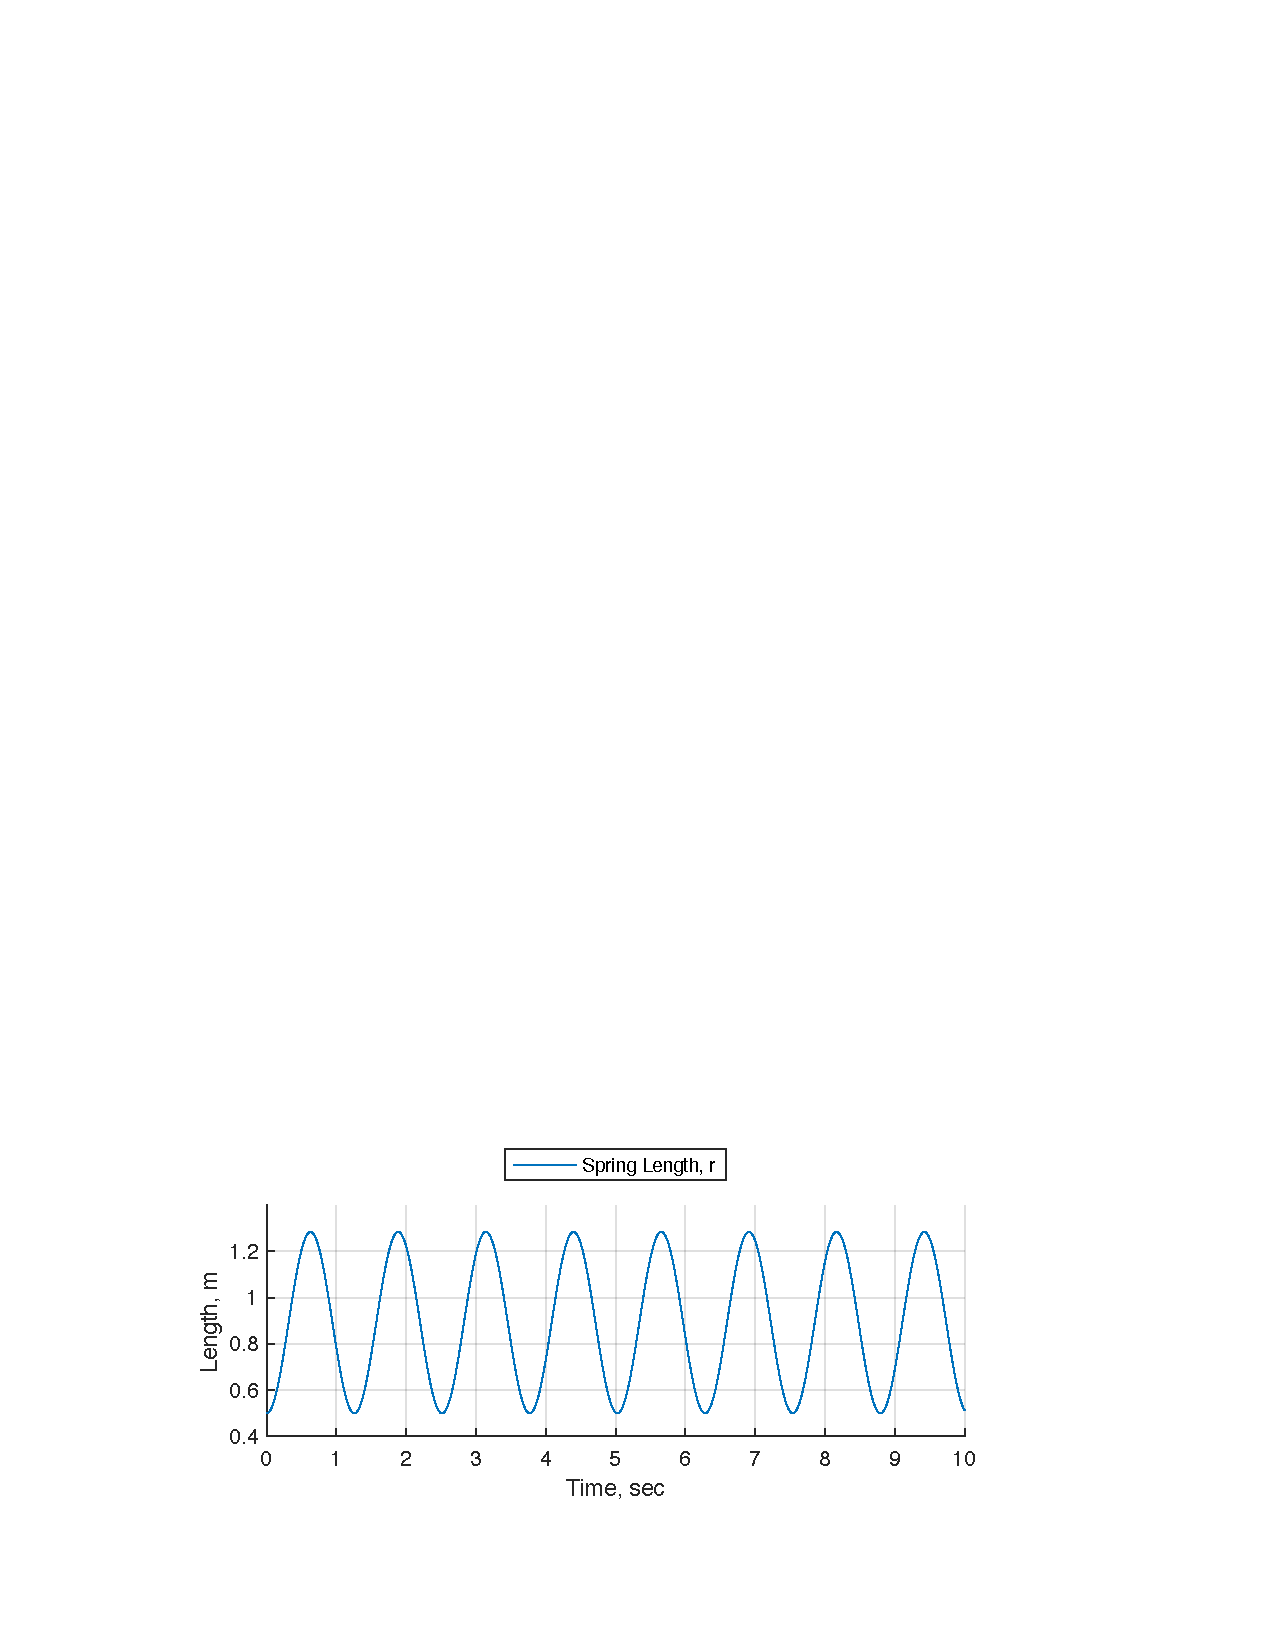
\includegraphics[center]{spring_0-0}
  \caption*{Spring Length vs. Time}
  \label{fig:spring:0:0}
\end{subfigure}
\end{figure}

The first configuration consists of the system being released from rest with no initial
angular deflection, and the spring at it's unstretched initial length; this configuration
therefore has no change in angular position, and simply begins to oscillate from the repeated
stretching of the spring.

\begin{figure}[!ht]
\caption{Numerical Solution Motion Behavior Plot, ($\theta_o:~\sfrac{\pi}{18},~\phi_o:~\sfrac{\pi}{9}$)}
\begin{subfigure}[t]{\textwidth}
  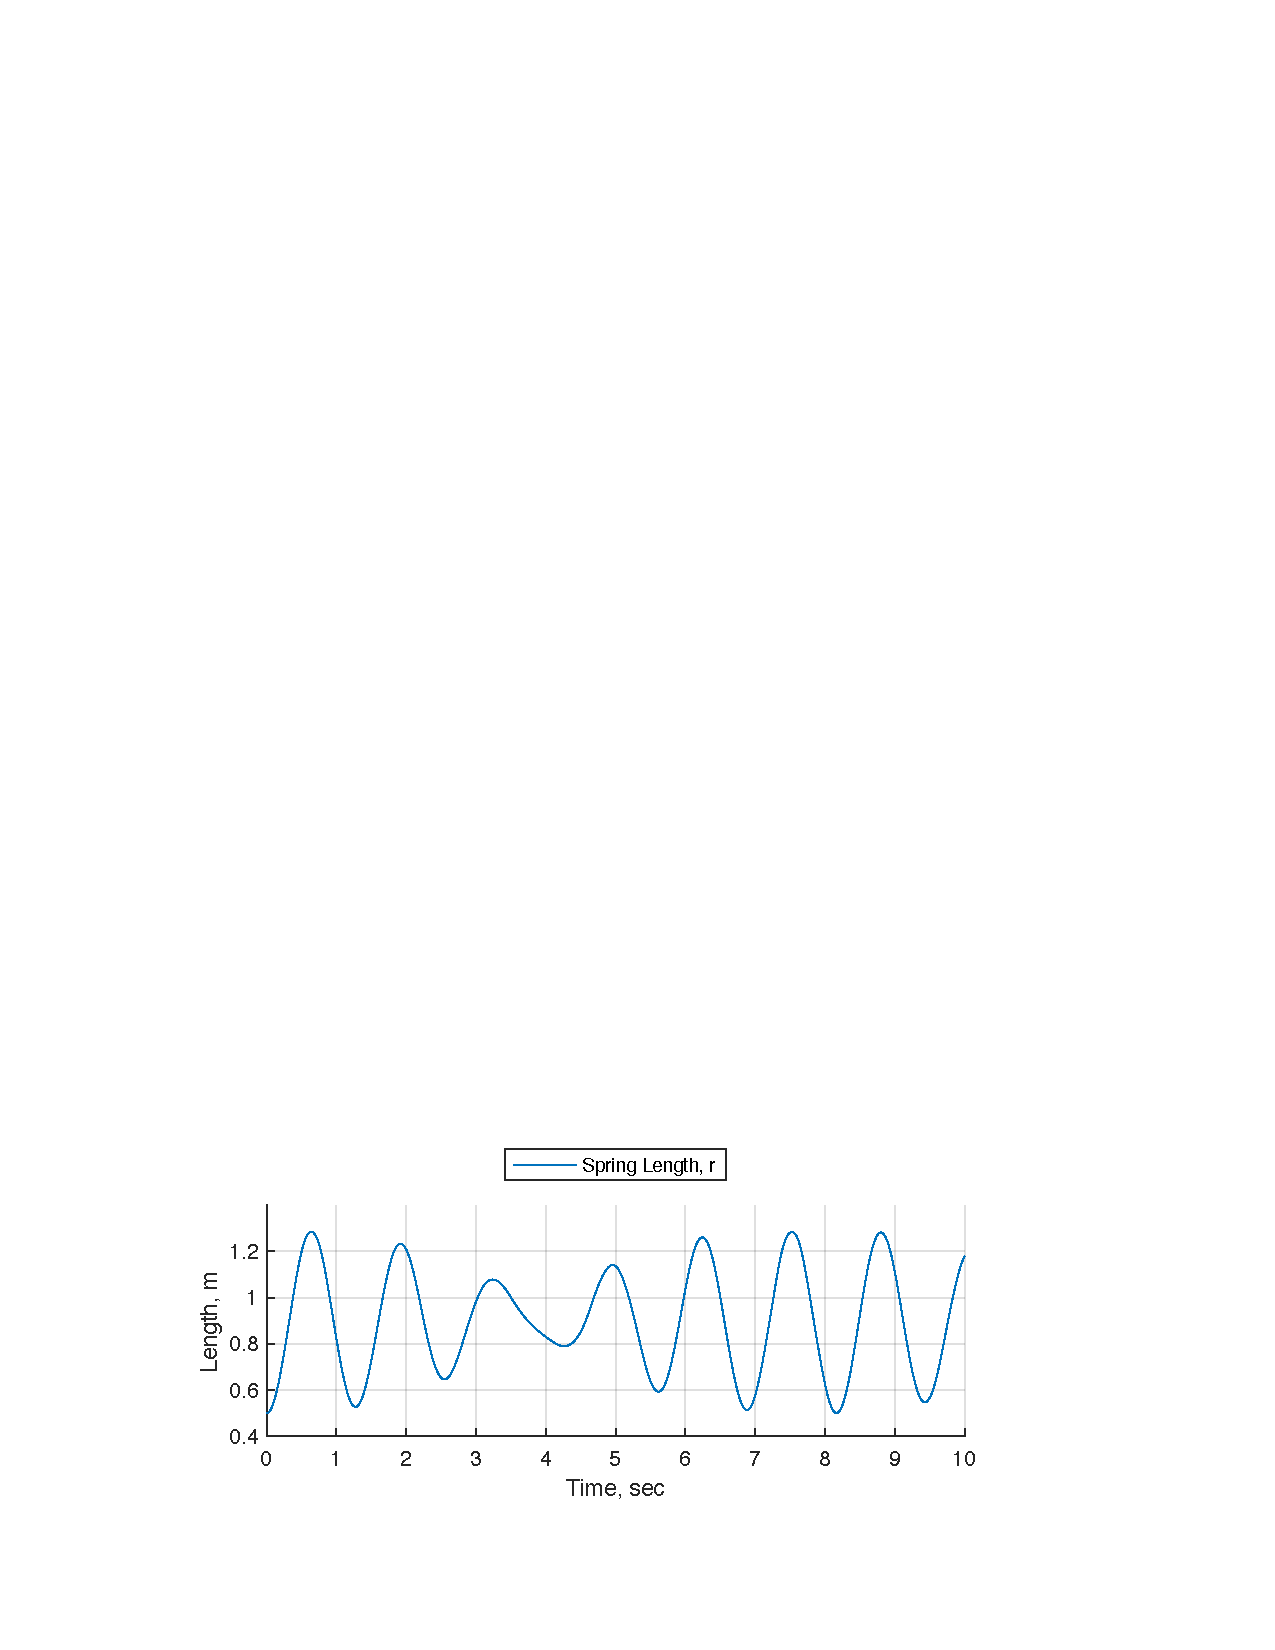
\includegraphics[center]{spring_18-9}
  \caption{Spring Length vs. Time}
  \label{fig:spring:18-9}
\end{subfigure}
\end{figure}
\begin{figure}[!ht] \ContinuedFloat
  \phantomcaption
\begin{subfigure}[t]{\textwidth}
  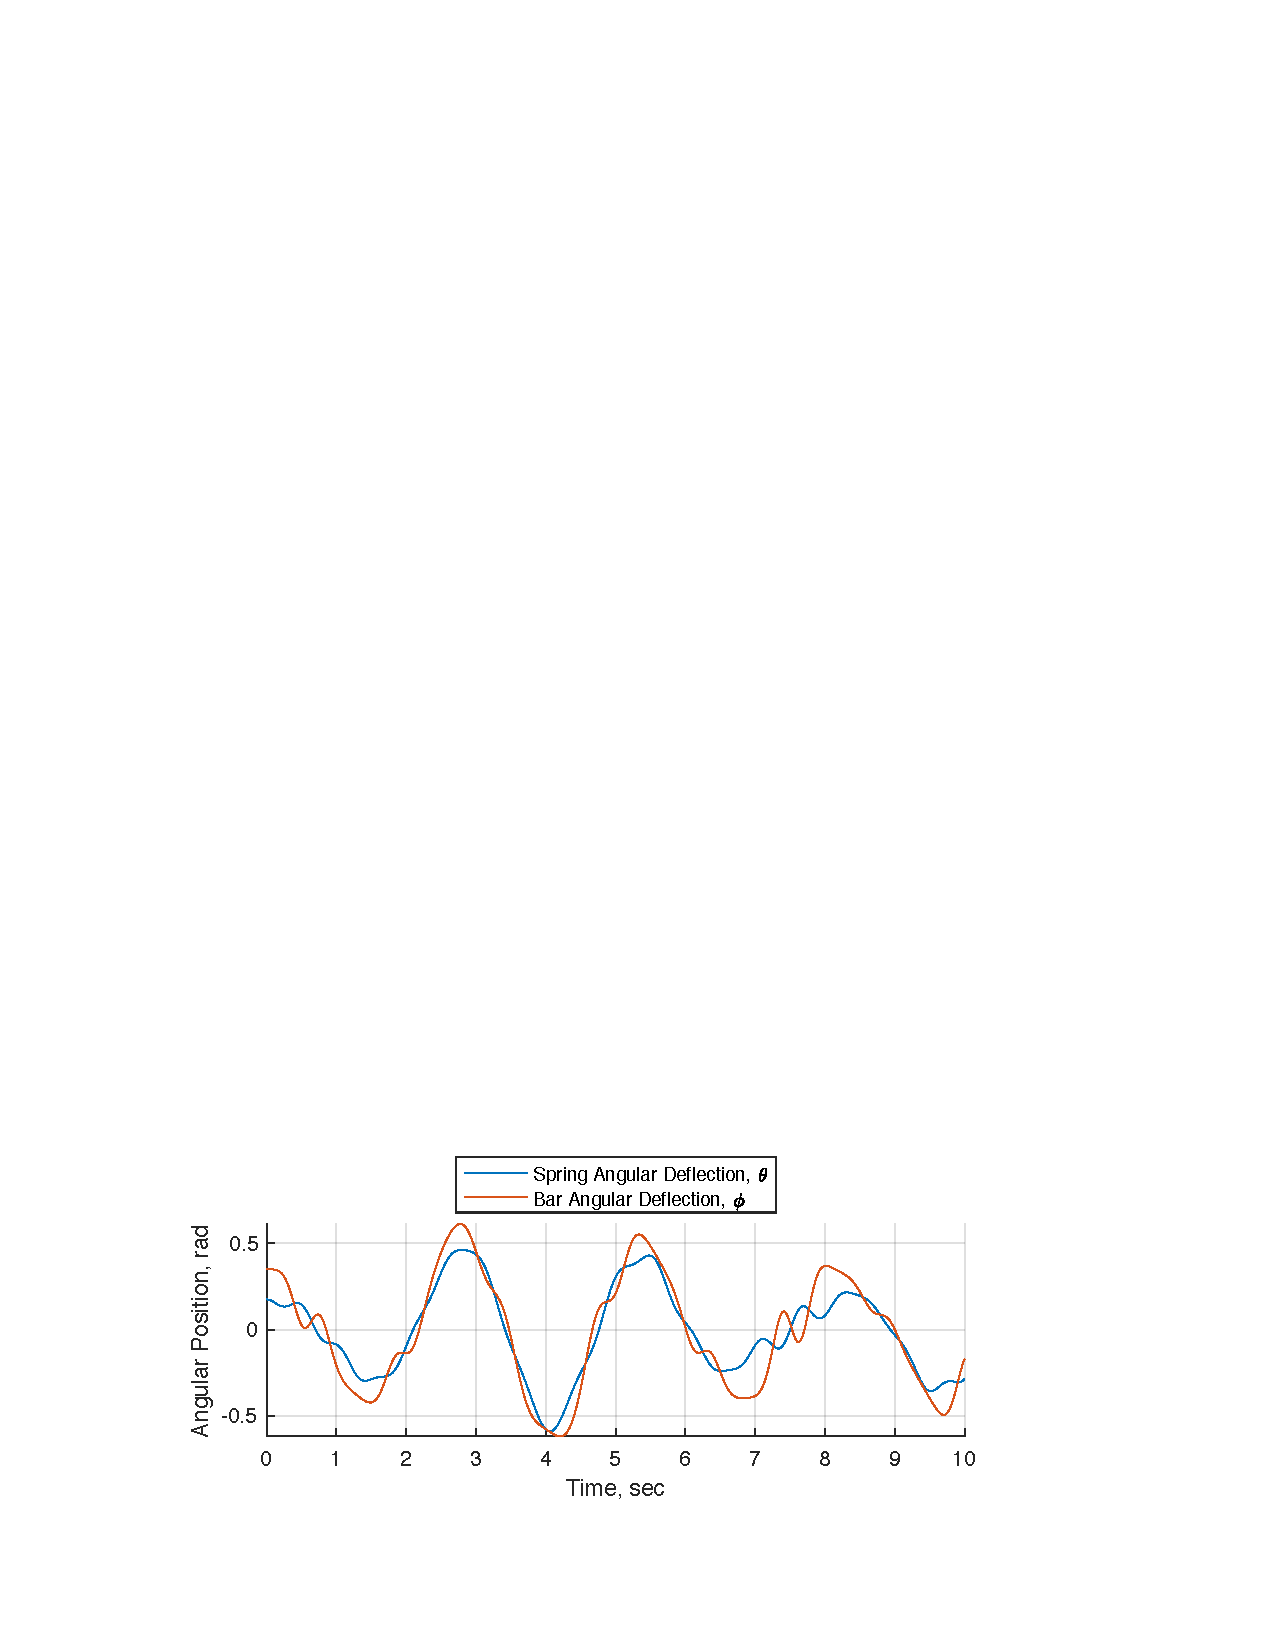
\includegraphics[center]{angles_18-9}
  \caption{Angular Position vs. Time}
  \label{fig:angles:18-9}
\end{subfigure}
\end{figure}
Figures (\ref{fig:spring:18-9}) and (\ref{fig:angles:18-9}) depict the behavior of the spring length as
well as angular deflection of the spring and bar, given the initial conditions shown.
Since the overall behavior in Figure (\ref{fig:angles:18-9}) is relatively consistent
(compared to that of Figure (\ref{fig:angles:6-3}) below), it makes sense that the spring
deflection plot depicts mostly consistent oscillatory motion -- since the amplitude in the
oscillations of the pendulum are smaller, there is less energy being "transferred," so-to-speak,
from the kinetic energy of the bar (force outward from the spring, dependent on it's velocity and acceleration)
to or from the energy in the spring. This phenomena can also be seen in Figure (\ref{fig:spring:6-3}), where the amplitudes
of oscillation in the spring deflection are larger relative to that of this situation, due to the fact that the
inital conditions in the case of Figure (\ref{fig:spring:6-3}) are of a greater
angular deflection. Given that the inital release angle
of the spring and bar are small (less than 45$^o$), the overall inital potential energy of the
system is lower, subsequently confirming the forementioned idea that there is less overall energy in the system,
as represented by the generally smaller amplitude in oscillations.
\begin{figure}[!ht]
\caption{Numerical Solution Motion Behavior Plot, ($\theta_o:~\sfrac{\pi}{6},~\phi_o:~\sfrac{\pi}{3}$)}
\begin{subfigure}[t]{\textwidth}
  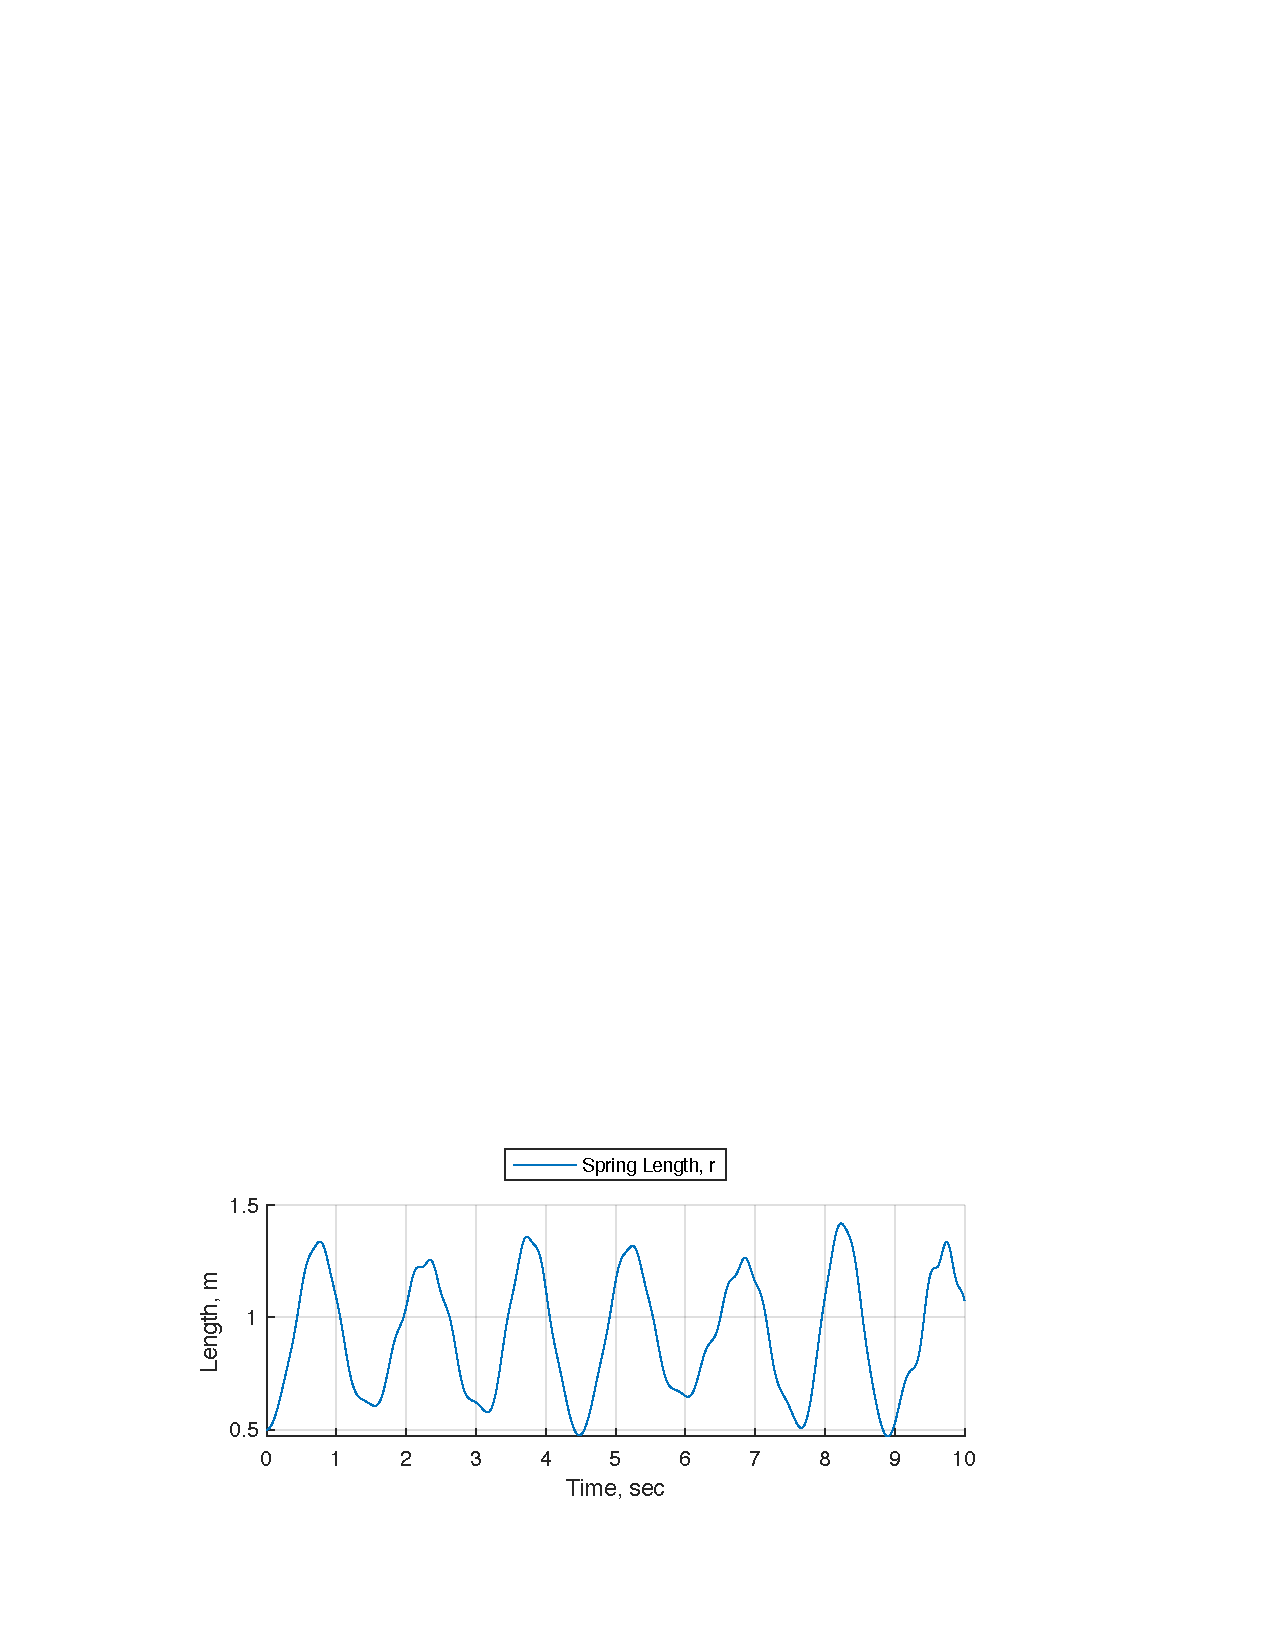
\includegraphics[center]{spring_6-3}
  \caption{Spring Length vs. Time}
  \label{fig:spring:6-3}
\end{subfigure}
\end{figure}
\begin{figure}[!ht] \ContinuedFloat
  \phantomcaption
\begin{subfigure}[t]{\textwidth}
  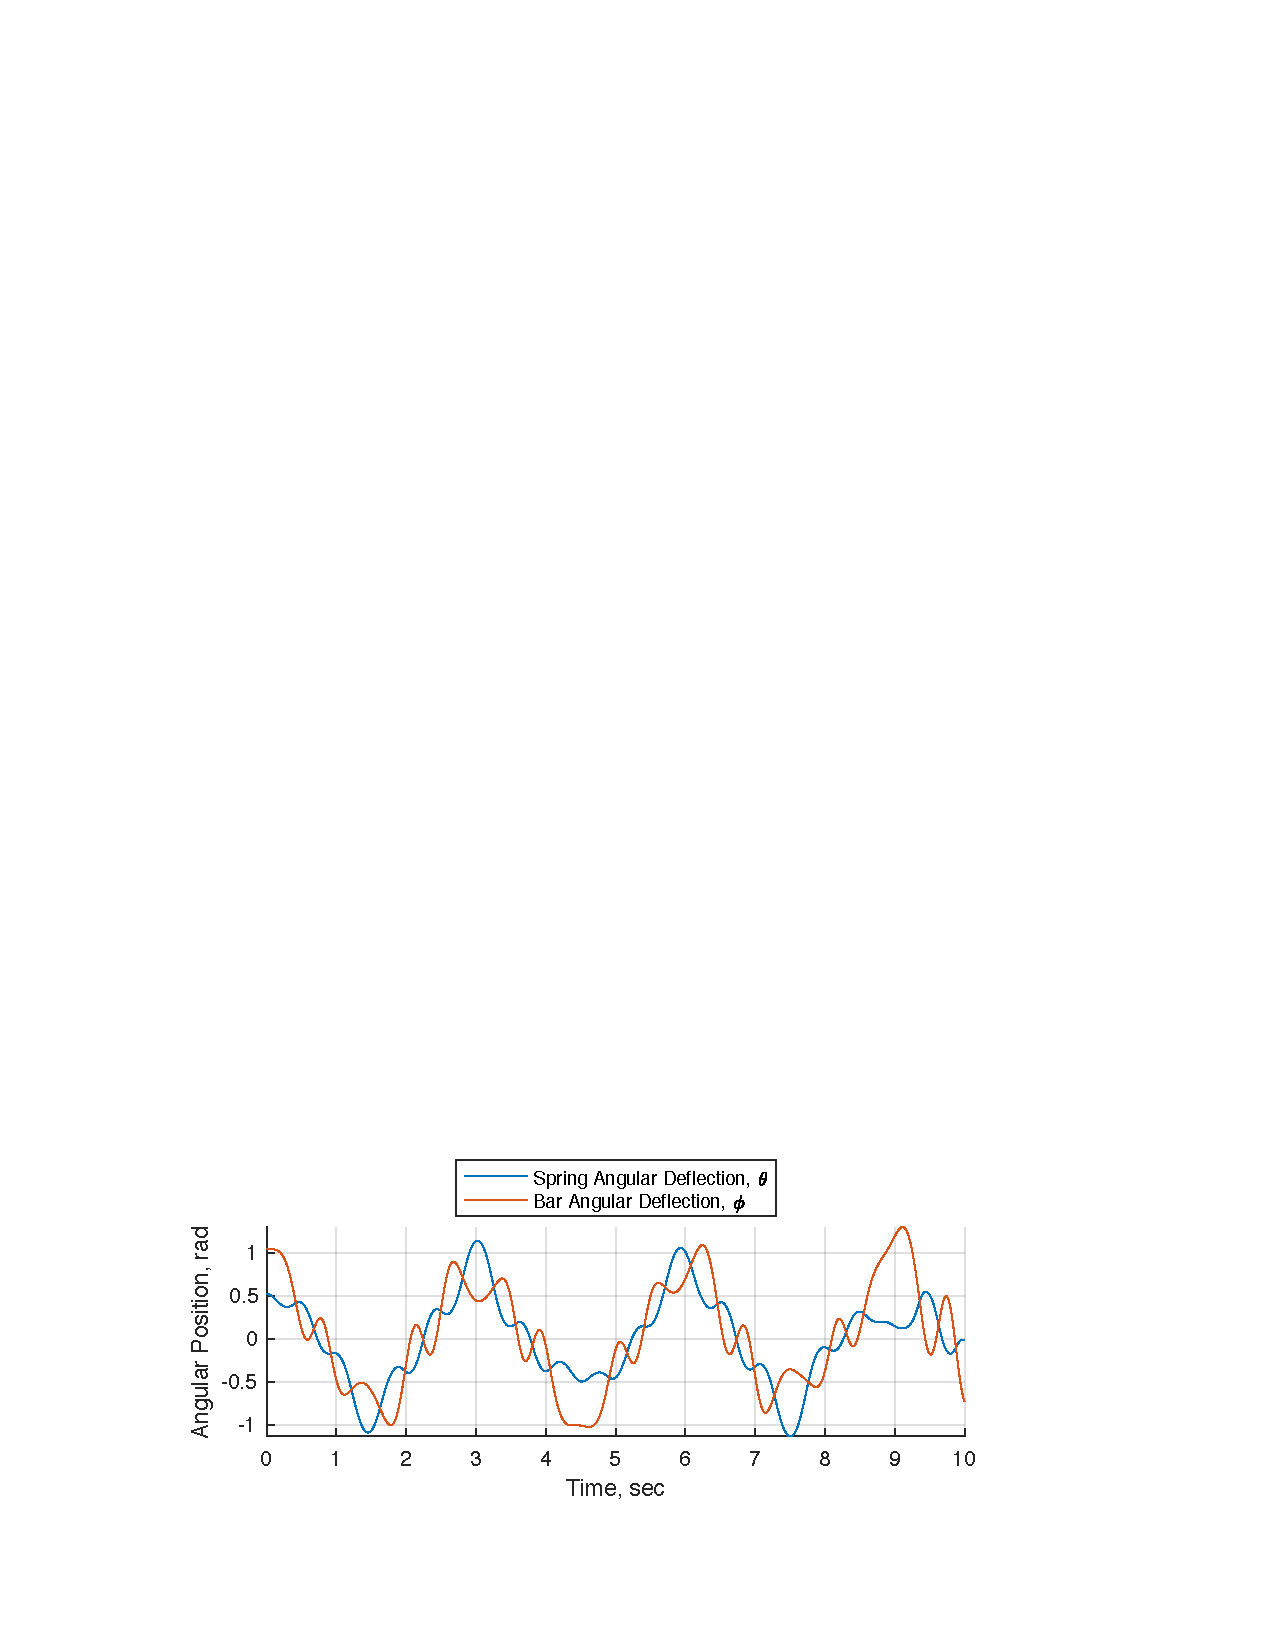
\includegraphics[center]{angles_6-3}
  \caption{Angular Position vs. Time}
  \label{fig:angles:6-3}
\end{subfigure}
\end{figure}


Figures (\ref{fig:spring:6-3}) and (\ref{fig:angles:6-3}) depict the behavior of the
system when released from larger inital angular deflections, as discussed previously,
introducing a larger initial potential energy, resulting in larger amplitudes of oscillation --
1 radian peak-to-peak in Figure (\ref{fig:angles:18-9}) compared to about 2 radians
peak-to-peak in Figure (\ref{fig:angles:6-3}); similarly, the magnitude of the spring
deflection is larger, going from a consistent 1.3 meters in Figure (\ref{fig:spring:18-9})
to almost 1.5 meters in Figure (\ref{fig:spring:6-3}).

\newpage

\begin{figure}[!htp]
  \caption{Total Energy Comparison Plots}
\begin{subfigure}[t]{\textwidth}
  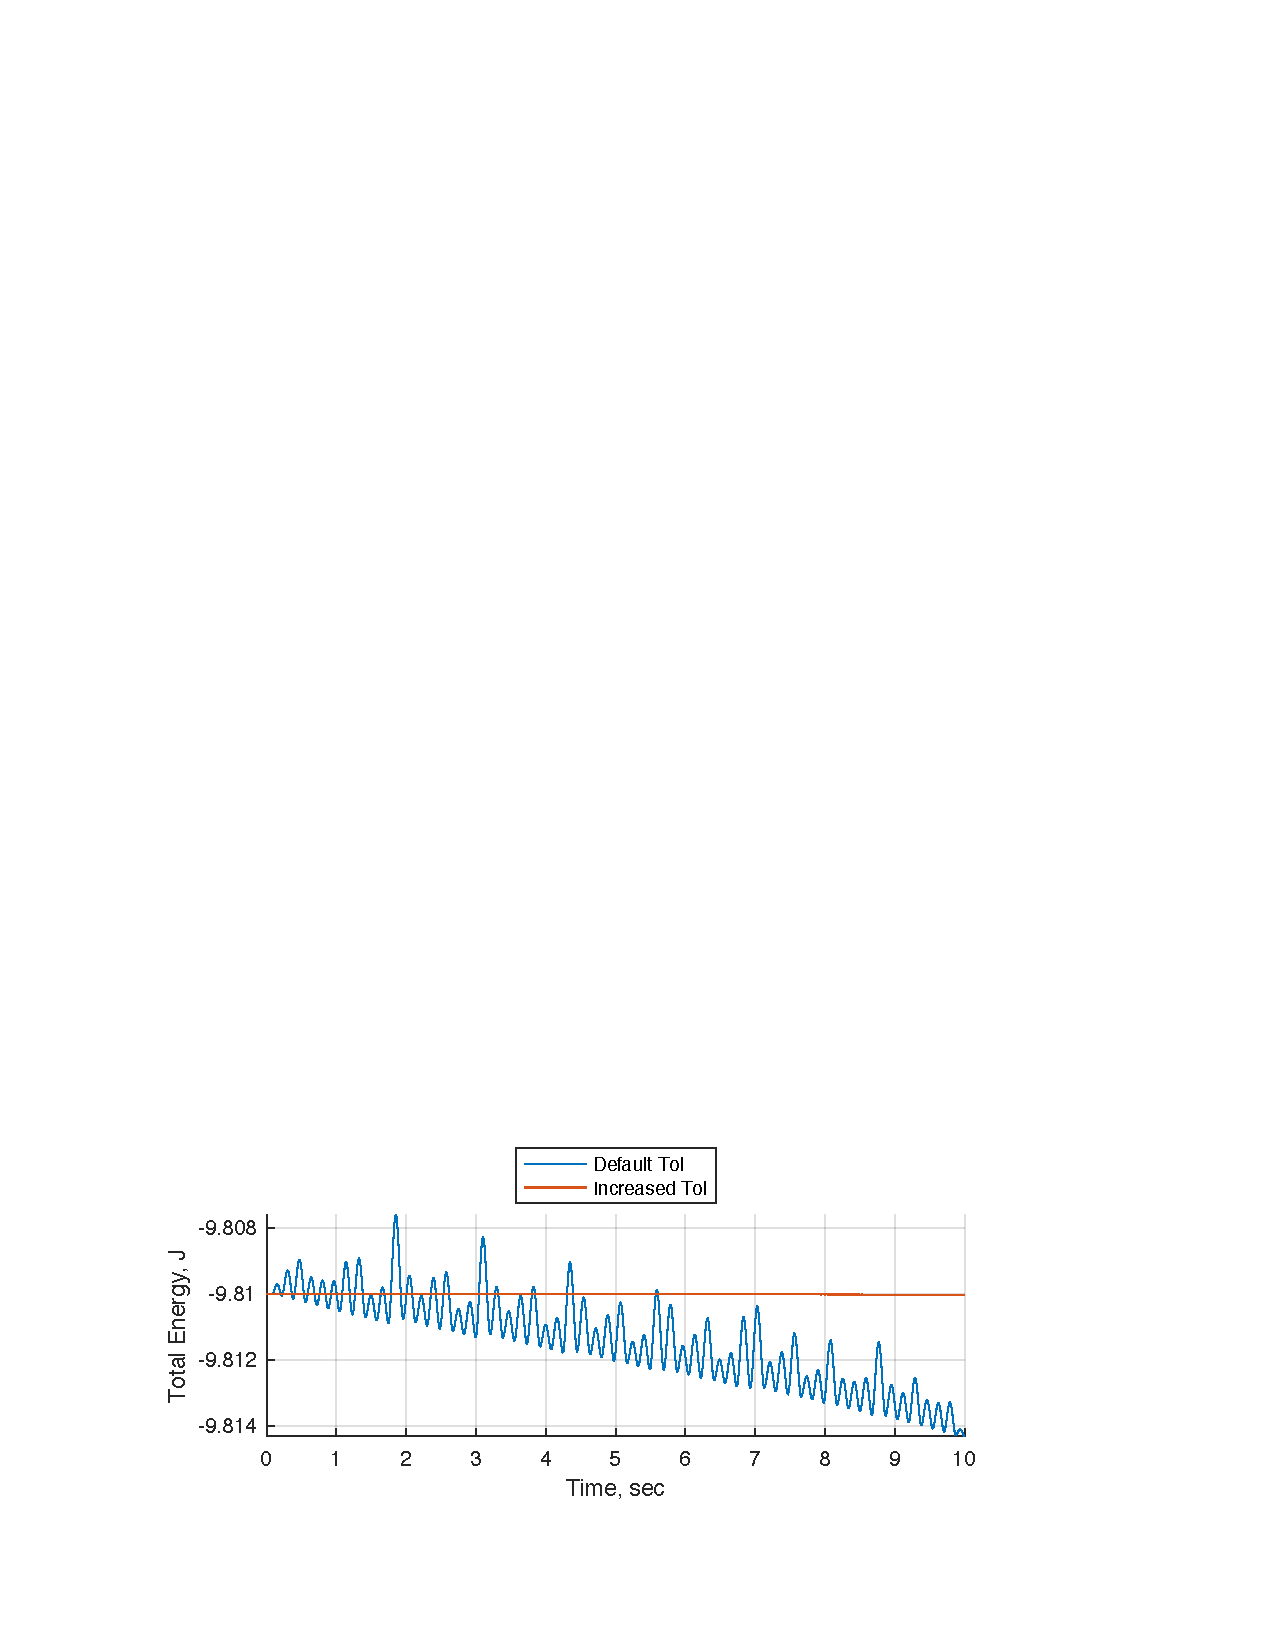
\includegraphics[center]{Energy1}
  \caption{Total Energy in the System ($\theta_o:0,~\phi_o:0$)}
  \label{fig:Energy1}
\end{subfigure}
\end{figure}
\null
\begin{figure}[!ht] \ContinuedFloat
  \phantomcaption
\begin{subfigure}[t]{\textwidth}
  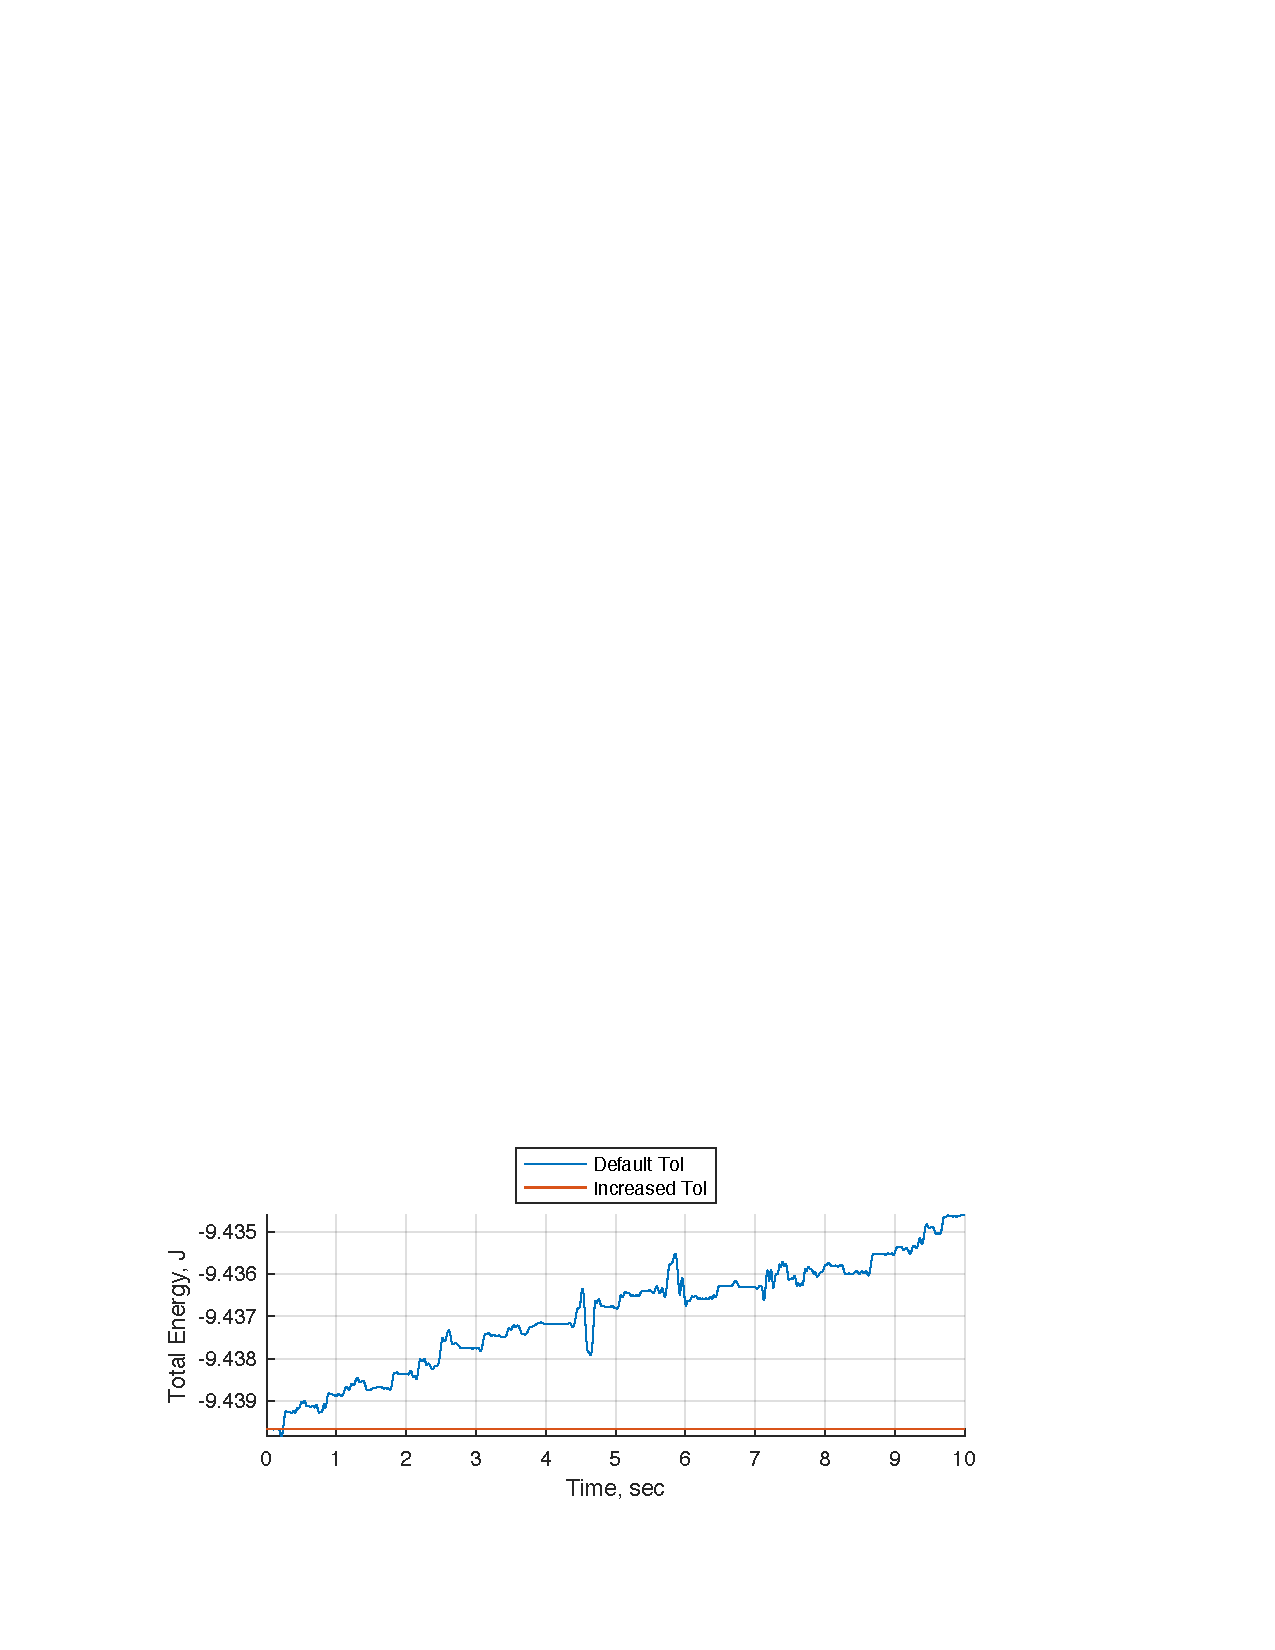
\includegraphics[center]{Energy2}
  \caption{Total Energy in the System ($\theta_o:~\sfrac{\pi}{18},~\phi_o:~\sfrac{\pi}{9}$)}
  \label{fig:Energy2}
\end{subfigure}
\end{figure}

\begin{figure}[!ht] \ContinuedFloat
  \phantomcaption
\begin{subfigure}[t]{\textwidth}
  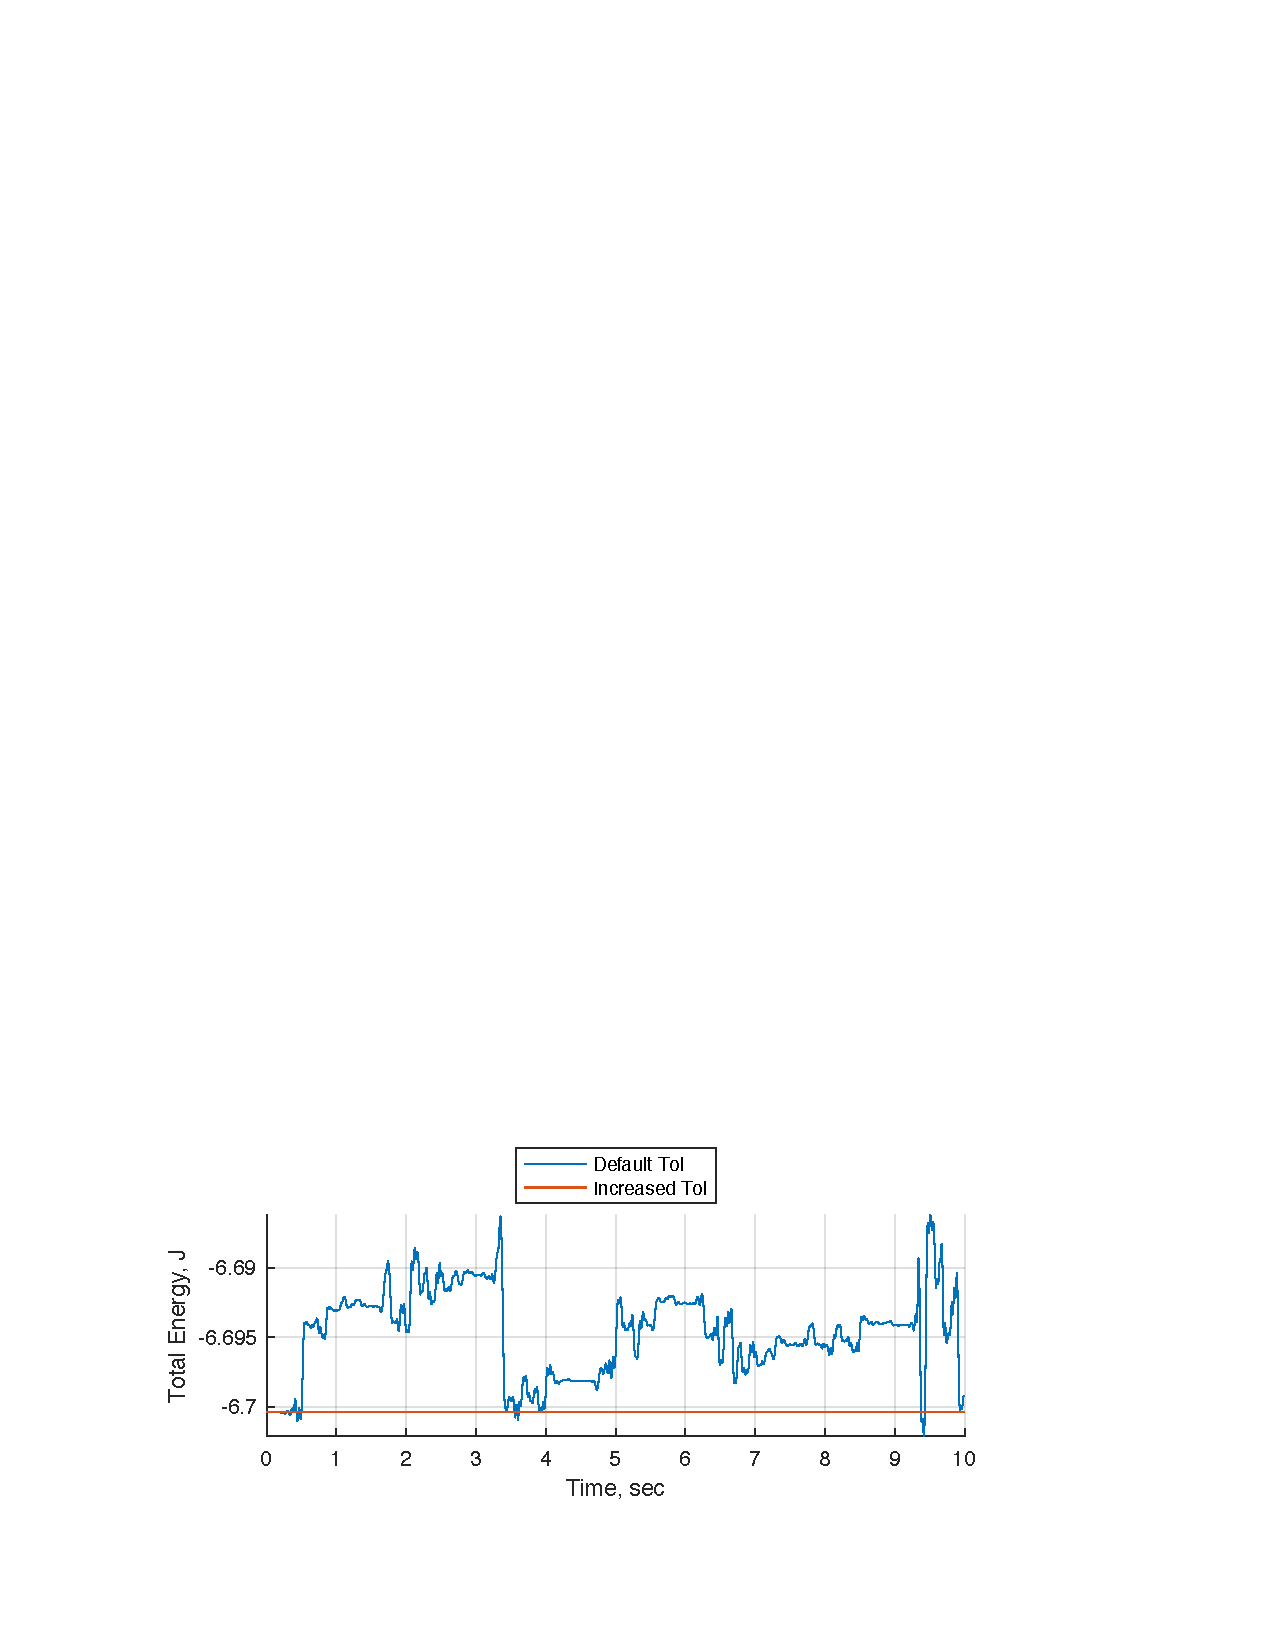
\includegraphics[center]{Energy3}
  \caption{Total Energy in the System ($\theta_o:~\sfrac{\pi}{6},~\phi_o:~\sfrac{\pi}{3}$)}
  \label{fig:Energy3}
\end{subfigure}
\end{figure}
\newpage
\flushleft
Running the |ode45| function with a relative tolerance of
$1*10^{-6}$ and an absolute
tolerance of $1*10^{-9}$ we produce a total energy graph that strays significantly
less than the default |ode45| implementation. The max percentage difference between
the high and low tolerance integrations in Figure (\ref{fig:Energy1}) is -0.0245\%.
The max percentage difference in Figure (\ref{fig:Energy2}) is
-0.0538\%. The max percentage difference in Figure (\ref{fig:Energy3}) is
-0.2116\%.

% ---------------------------------------------------------------------------- %
\newpage
\section{Does it Make Sense?}
% ---------------------------------------------------------------------------- %

\subsection{Units}
Checking with the MATLAB symbolic units tool (from Section \ref{appendix:numerical}): \\
~\\
\begin{lstlisting}[frame=lines,style=Matlab-editor]
% Checking EOM Units
u = symunit;
m2 = m2*u.kg;
k = k*u.N/u.m;
L0 = L0*u.m;
l2 = l2*u.m;
g = g*u.m/u.s^2;
thetat = 'thetat';
thetadot = 'thetadot'/u.s;
thetaddot = 'thetaddot'/u.s^2;
phit = 'phit';
phidot = 'phidot'/u.s;
phiddot = 'phiddot'/u.s^2;
l1t = 'l1t'*u.m;
l1dot = 'l1dot'*u.m/u.s;
l1ddot = 'l1ddot'*u.m/u.s^2;

eqn = subs(eqn)
unitCheck = checkUnits(eqn)
\end{lstlisting}
\color{gray} \begin{verbatim}
unitCheck =
  struct with fields:
    Consistent: [1 1 1]
    Compatible: [1 1 1]
\end{verbatim} \color{black}

\subsection{Magnitude}
Examining the figures we can see that the magnitude of spring length never exceeds the max length achieved in the first period. This indicated that no energy is added in the spring oscillation, which is expected due to the fact that we have no external forces affecting the spring-bar system. Similarly, figures
(\ref{fig:Energy1}), (\ref{fig:Energy2}), and (\ref{fig:Energy3}) all indicate that the total energy within the system remains essentially constant. There is a minor drift in the total energy on the magnitude of $10^{-3}J$ for our loosly toleranced integrations. With the more highly toleranced integrations the energy drift is on the magnitude of $10^{-6}$. This low change in energy relative tot he total energy of the system indicates that the conservation of energy principle holds true in our system that lacks non-conservative forces.
\section{Appendix} \label{appendix}
\subsection{Attributions}
\onehalfspacing
\begin{tabular}{ll}
Jeffrey Chen & \\
Thorne Wolfenbarger & \\
Trey Dufrene & \\
Joint Effort &
\end{tabular}
\singlespacing

\newpage
\subsection{Analytical Solution}

\newpage
\subsection{Numerical Solution} \label{appendix:numerical}
% \begin{lstlisting}[frame=lines,style=Matlab-editor,basicstyle = \mlttfamily]

\end{lstlisting}

% TODO: Add scan of Thorne's work? TODO TODO TODO TODO TODO TODO TODO TODO TODO TODO TODO TODO TODO TODO TODO TODO TODO TODO TODO TODO TODO TODO TODO TODO TODO
\begin{figure}[!htp]
  \caption{Comparison Plots of ode45 Tolerance Options}
  \begin{subfigure}{\textwidth}
    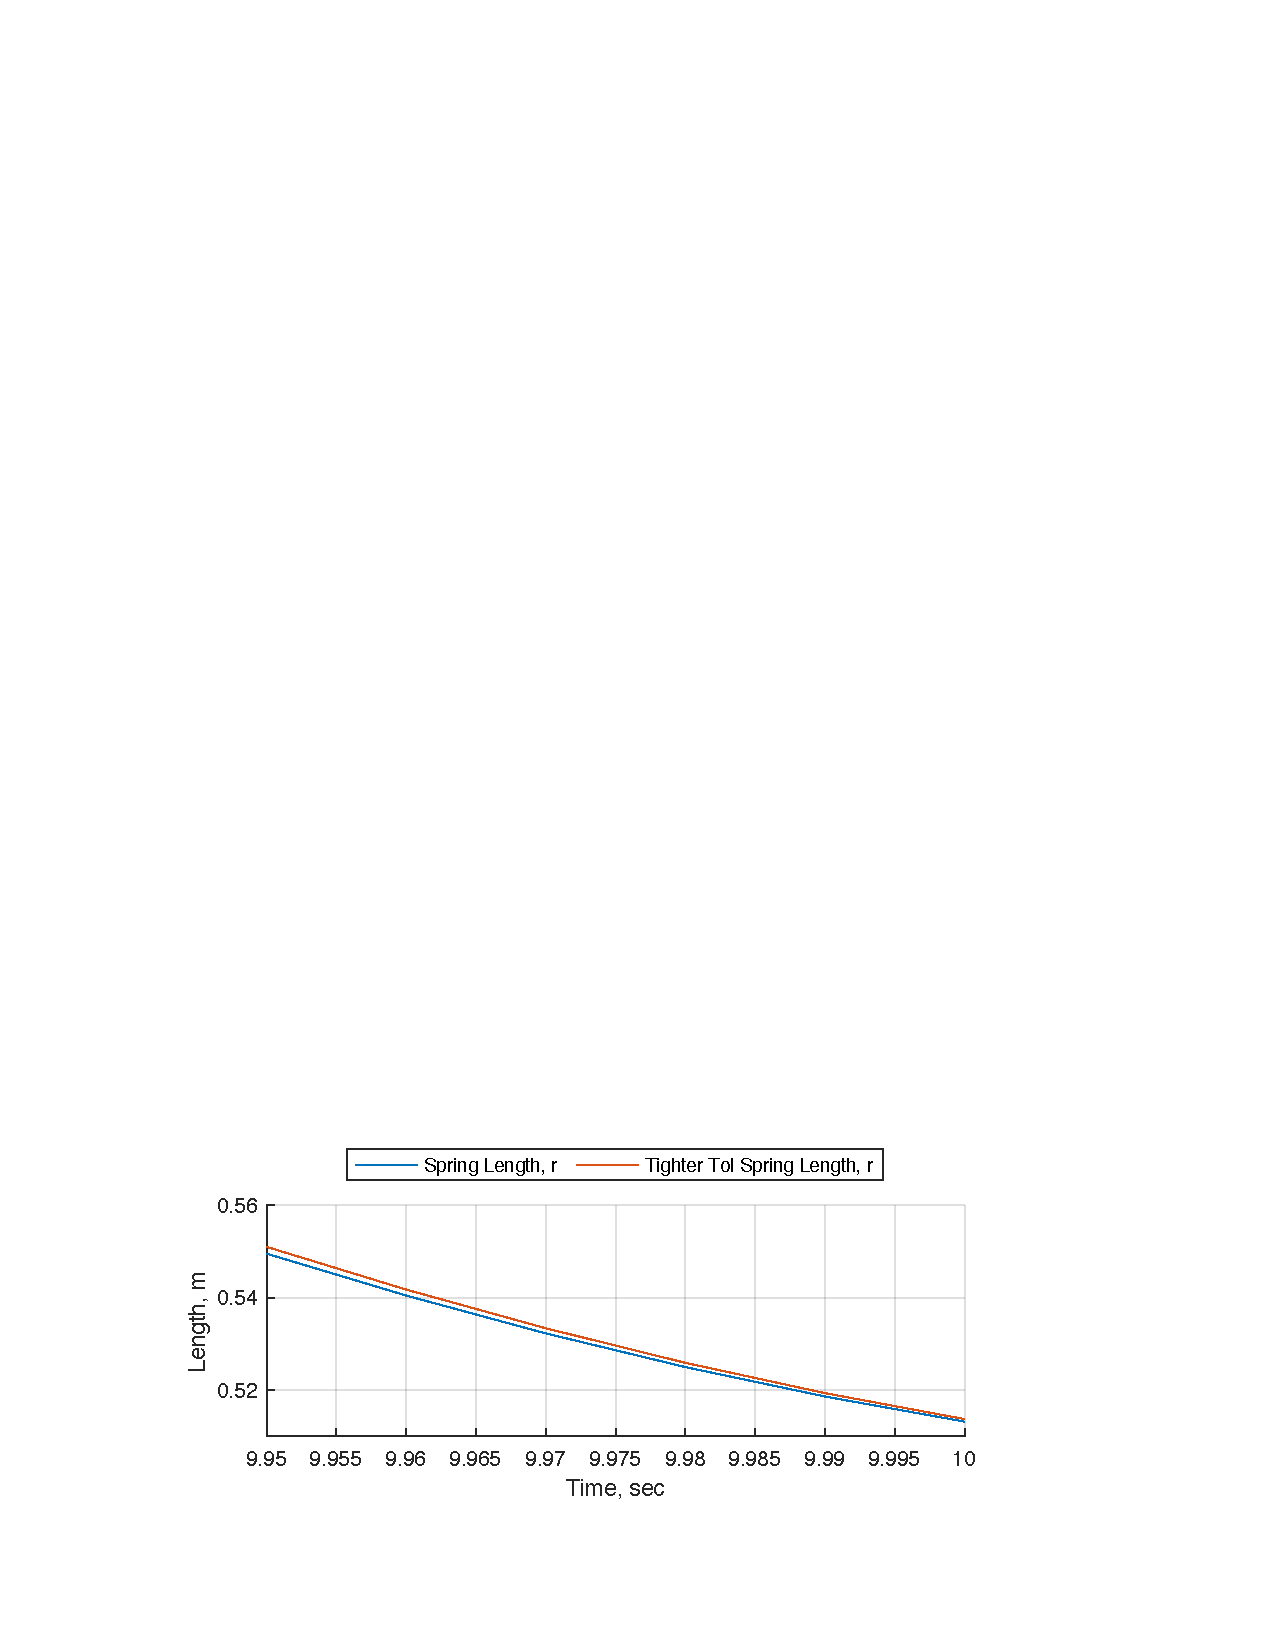
\includegraphics[center]{1}
    \caption*{Spring Deflection, ($\theta_o:~0,~\phi_o:~0$)}
  \end{subfigure}
  \begin{subfigure}{\textwidth}
    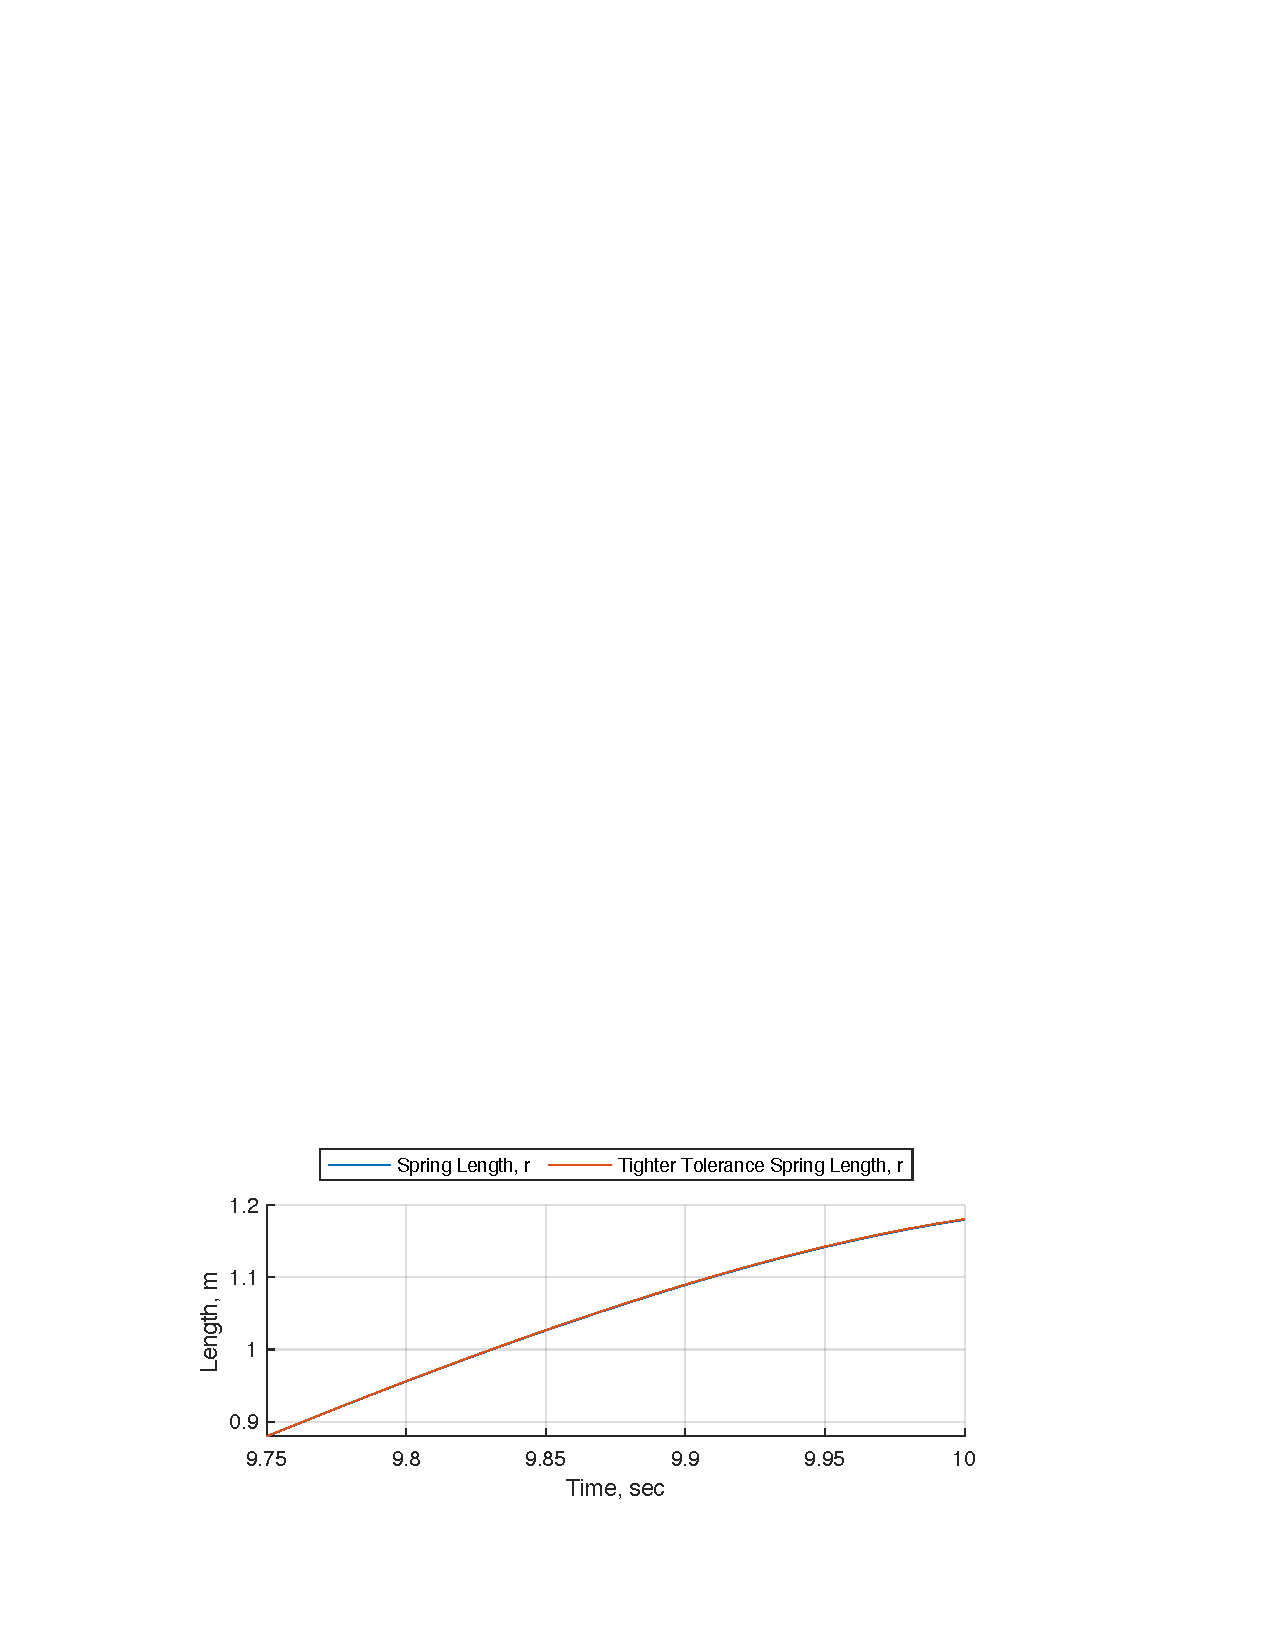
\includegraphics[center]{2}
    \caption*{Spring Deflection, ($\theta_o:\sfrac{\pi}{18},~\phi_o:\sfrac{\pi}{9}$)}
  \end{subfigure}
  \begin{subfigure}{\textwidth}
    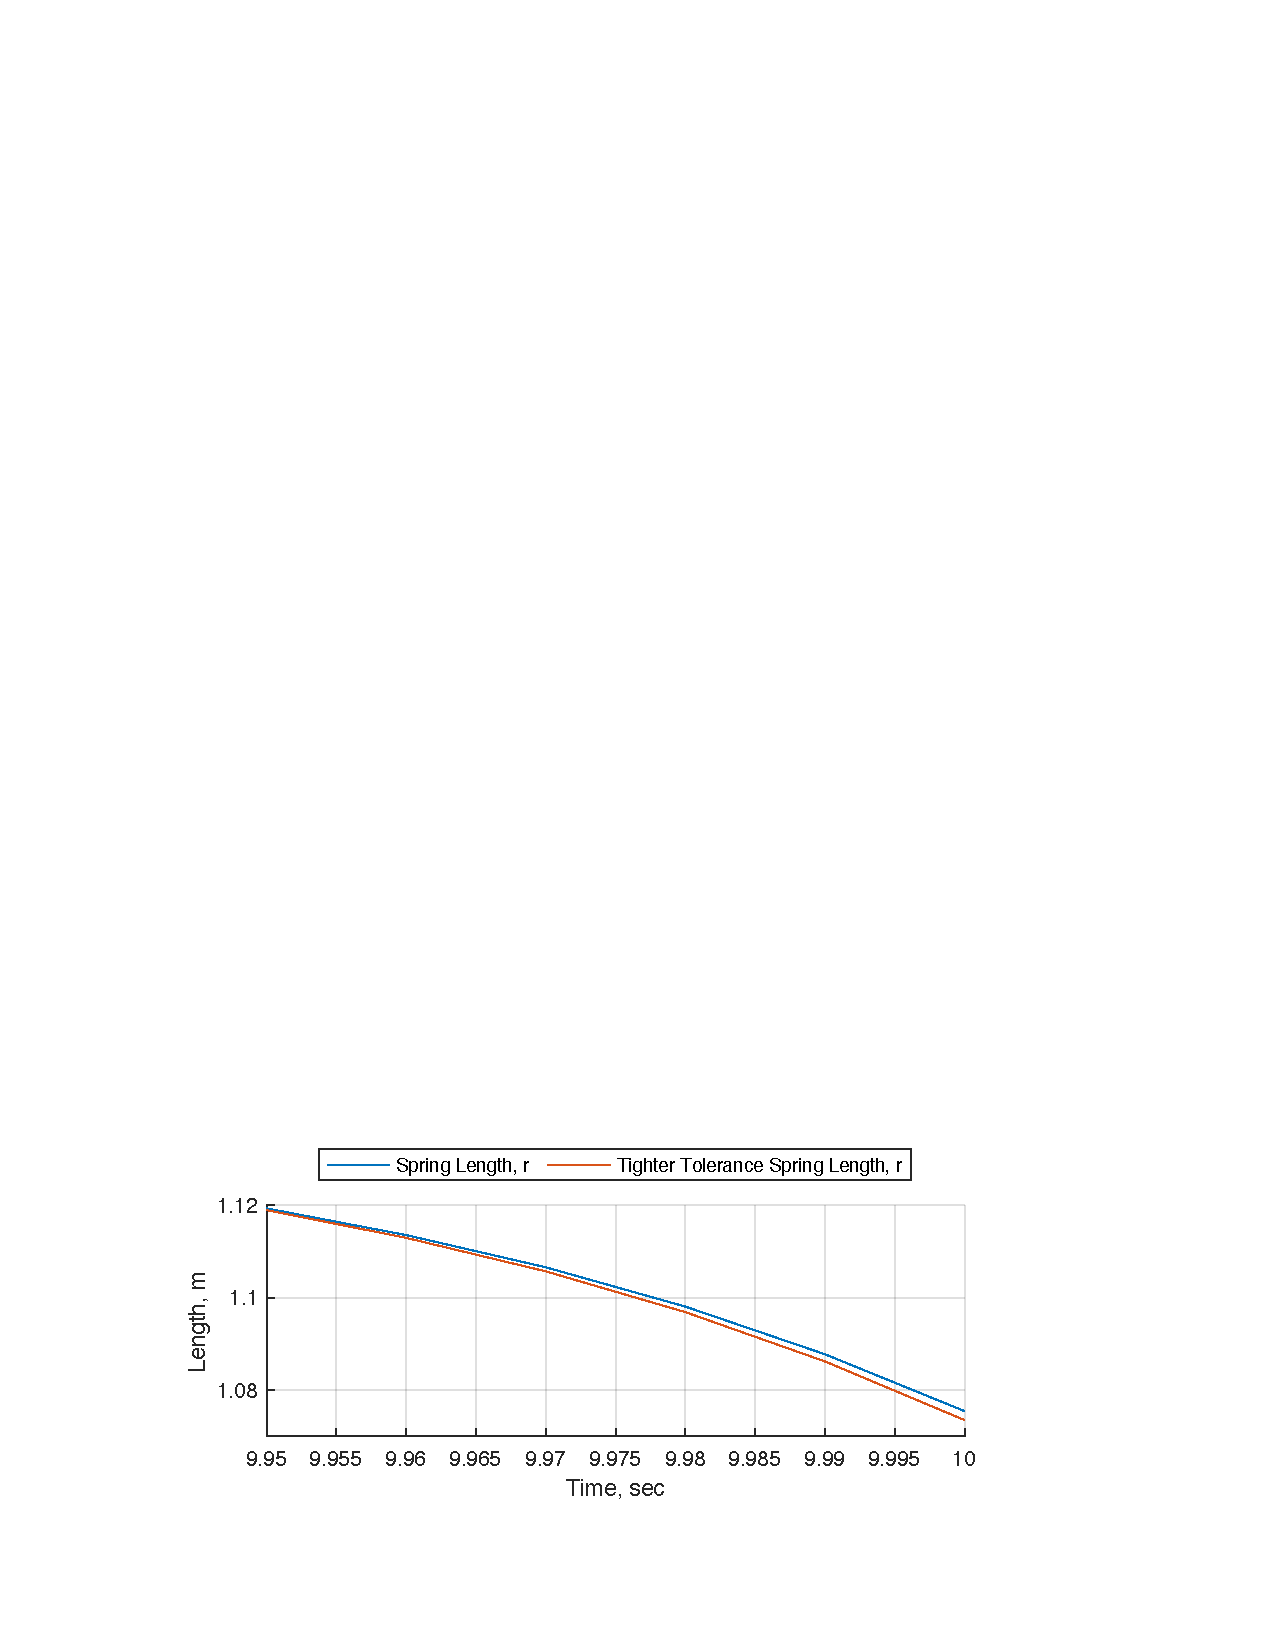
\includegraphics[center]{4}
    \caption*{Spring Deflection, ($\theta_o:\sfrac{\pi}{6},~\phi_o:\sfrac{\pi}{3}$)}
  \end{subfigure}
\end{figure}
\begin{figure}[!htp] \ContinuedFloat
  \begin{subfigure}{\textwidth}
    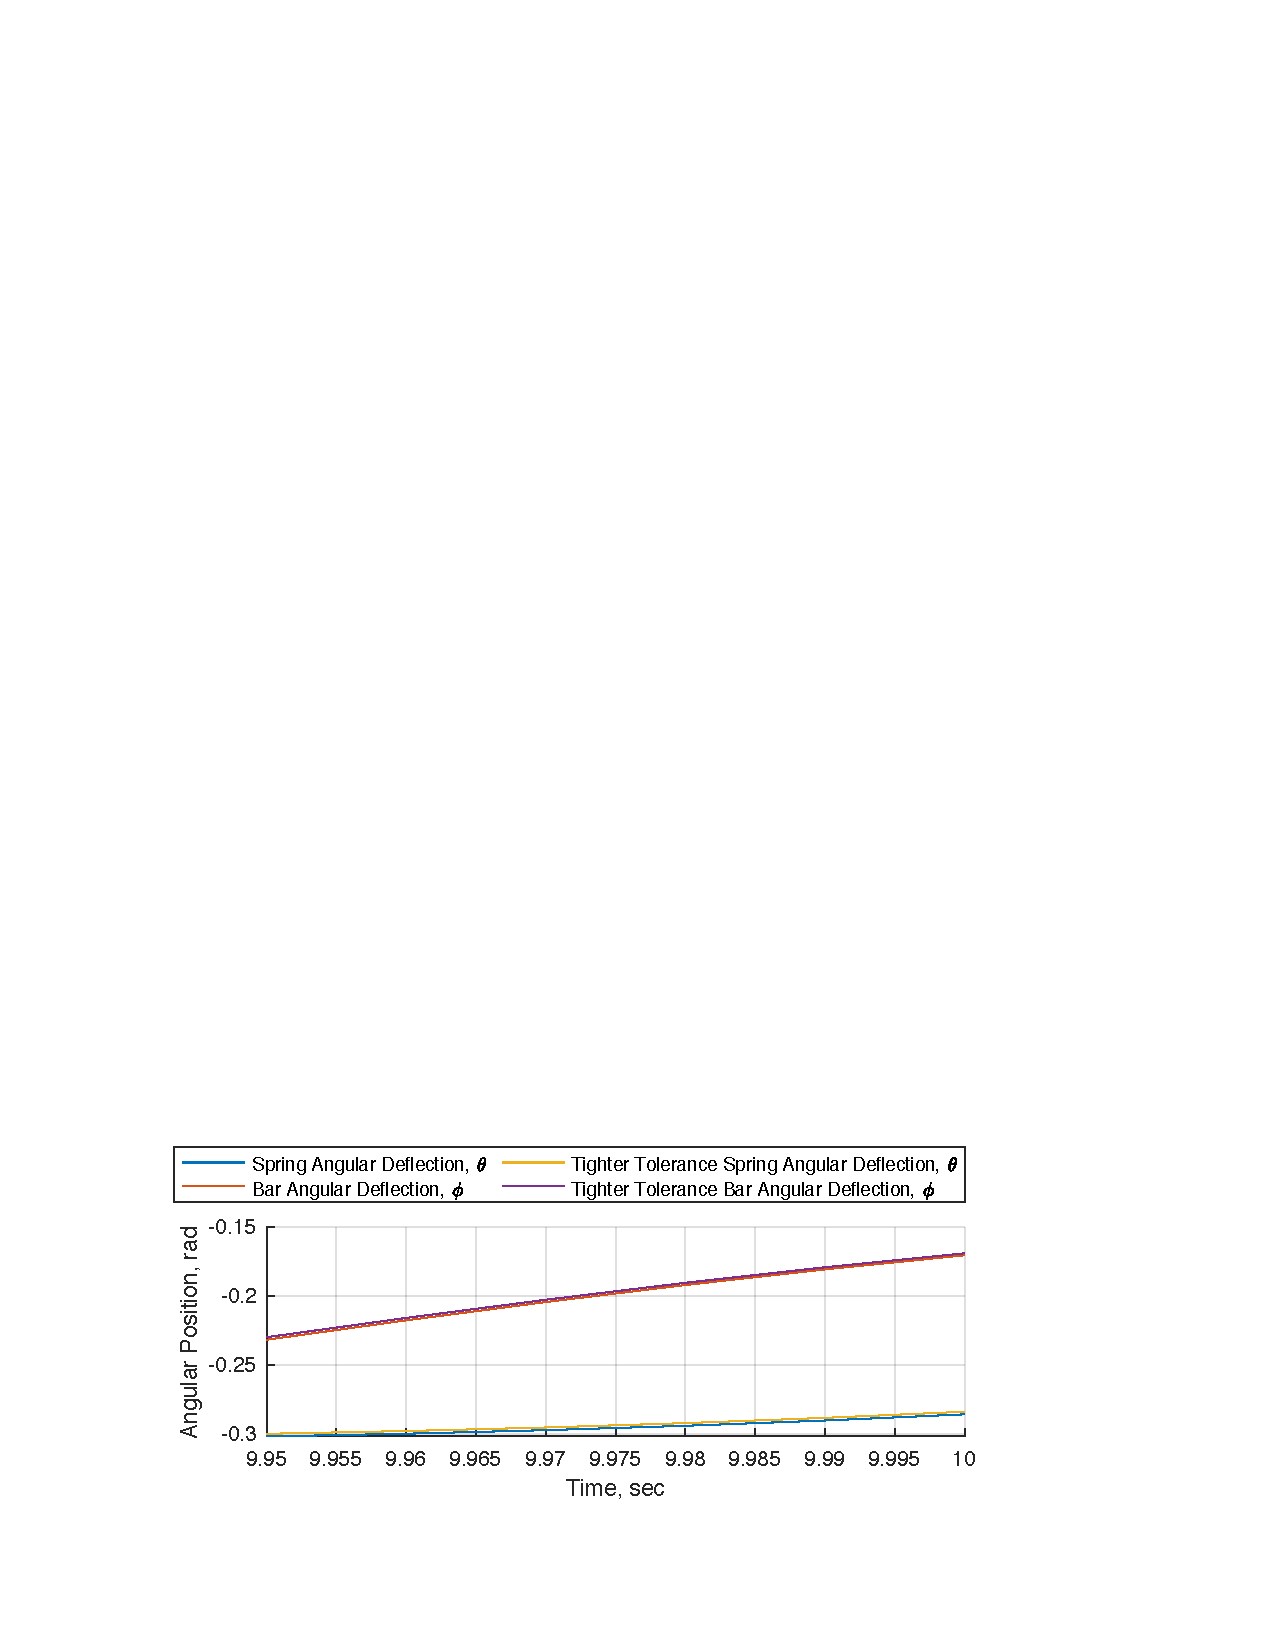
\includegraphics[center]{3}
    \caption*{Bar and Spring Angular Deflection, ($\theta_o:\sfrac{\pi}{18},~\phi_o:\sfrac{\pi}{9}$)}
  \end{subfigure}
  \begin{subfigure}{\textwidth}
    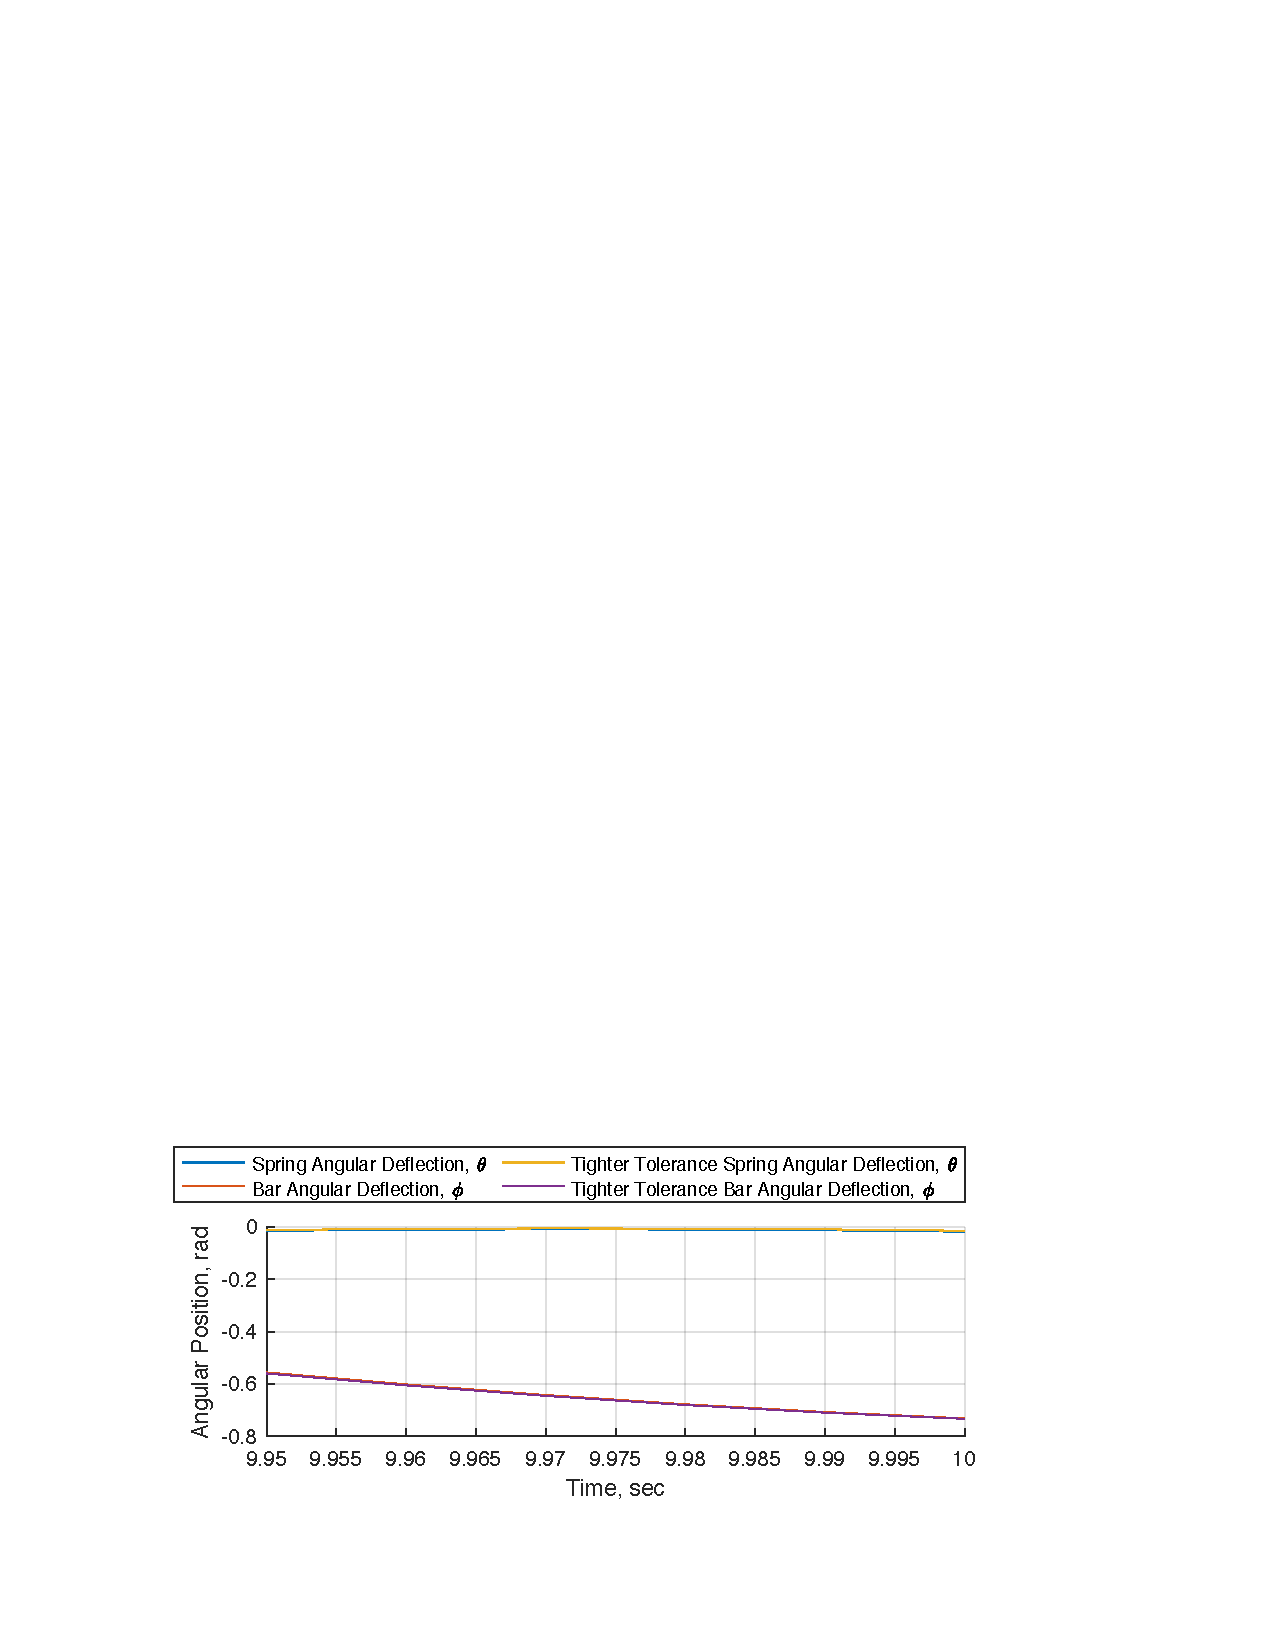
\includegraphics[center]{5}
    \caption*{Bar and Spring Angular Deflection, ($\theta_o:\sfrac{\pi}{6},~\phi_o:\sfrac{\pi}{3}$)}
  \end{subfigure}
\end{figure}


\end{flushleft}
\end{document}
